\documentclass[xcolor=dvipsnames]{beamer}
\usetheme{Madrid}


\setbeamertemplate{navigation symbols}{}
%\setbeamertemplate{headline}{}

%\setbeamertemplate{frametitle}{\insertpagenumber}
\setbeamertemplate{footline}[frame number]
%\setbeamersize{text margin left=7mm}
%\setbeamersize{text margin right=7mm}

\usepackage{colortbl}

\usepackage{hyperref}
%\hypersetup{colorlinks, linkcolor=black}
%\hypersetup{colorlinks,breaklinks}


\usepackage{times}

\usepackage{xltxtra}
\setsansfont{Calibri}
\setmonofont{Consolas}

\usepackage{minted}


\author{Jan Dědek}

\institute[MFF UK] % (optional, but mostly needed)
{
  Department of Software Engineering\\
	Faculty of Mathematics and Physics\\
	Charles University in Prague
}

\date[DEDEK-PHD, 2012]
{
Defence of Doctoral Thesis\\21\textsuperscript{st} September\\2012
}

\title{Semantic Annotations}

\begin{document}

\begin{frame}
  \titlepage
\end{frame}

\definecolor{DarkGreen}{rgb}{0,.392,0}
\definecolor{DarkMagenta}{rgb}{.545,0,.545}
\definecolor{DarkCyan}{rgb}{0,.545,.545}


\def \colorManual    {Brown}
\def \colorLearning  {DarkGreen}
\def \colorShareable {DarkCyan}
\def \colorFuzzy     {DarkMagenta}
\def \mysetbeamercolor [#1]#2 {\setbeamercolor{#1}{fg=#2}}

\mysetbeamercolor[colorManual]{\colorManual}
\mysetbeamercolor[colorLearning]{\colorLearning}
\mysetbeamercolor[colorShareable]{\colorShareable}
\mysetbeamercolor[colorFuzzy]{\colorFuzzy}


\def \themecolor #1 {\setbeamercolor*{titlelike}{parent=palette primary, bg=#1}}
\def \themetext [#1]#2 {{\usebeamercolor{#1}{\color{fg}\textbf{#2}}}}
\def \resetcolor {\setbeamercolor*{titlelike}{parent=palette primary}}



\definecolor{mybkg}{RGB}{240,240,240}
\setbeamercolor{block title}{bg=OliveGreen}
\setbeamercolor{block body}{bg=mybkg}

\begin{frame}{Outline}
  \tableofcontents
\end{frame}

\section{Introduction} 
\subsection{Information Extraction} 
\frame{\tableofcontents[currentsection, currentsubsection]}
\begin{frame}{Information Extraction (Problem)}  
\begin{itemize}
	\item Let's have a text describing an acquisition event.
	\medskip
	\framebox{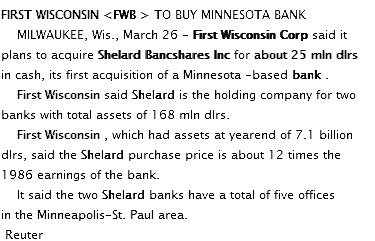
\includegraphics[width=0.6\hsize]{img/acquisitions_plain.png}}
	\item What was the object of the acquisition?
	\item Who was the buyer?
	\item What was the deal amount?
\end{itemize}
\end{frame}

\begin{frame}{Information Extraction (Solution)}  
\begin{itemize}
	\item Information Extraction tools can identify and extract such information.
	%\begin{itemize}
		%\item Of course not 100\% accurete...
	%\end{itemize}
	\bigskip	
	\begin{center}
	\framebox{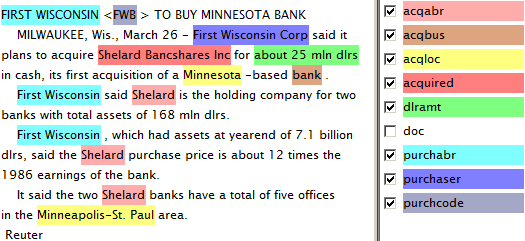
\includegraphics[width=0.85\hsize]{img/acquisitions_annotated.png}}
	\end{center}	
	%\item The tools can also interpret such information in terms of a \alert{Semantic Web Ontology}.
\end{itemize}
\end{frame}

\begin{frame}{Information Extraction (Czech Example)}  
\begin{itemize}
	\item Information Extraction tools can identify and extract such information.
	%\begin{itemize}
		%\item Of course not 100\% accurete...
	%\end{itemize}
	\bigskip	
	\begin{center}
	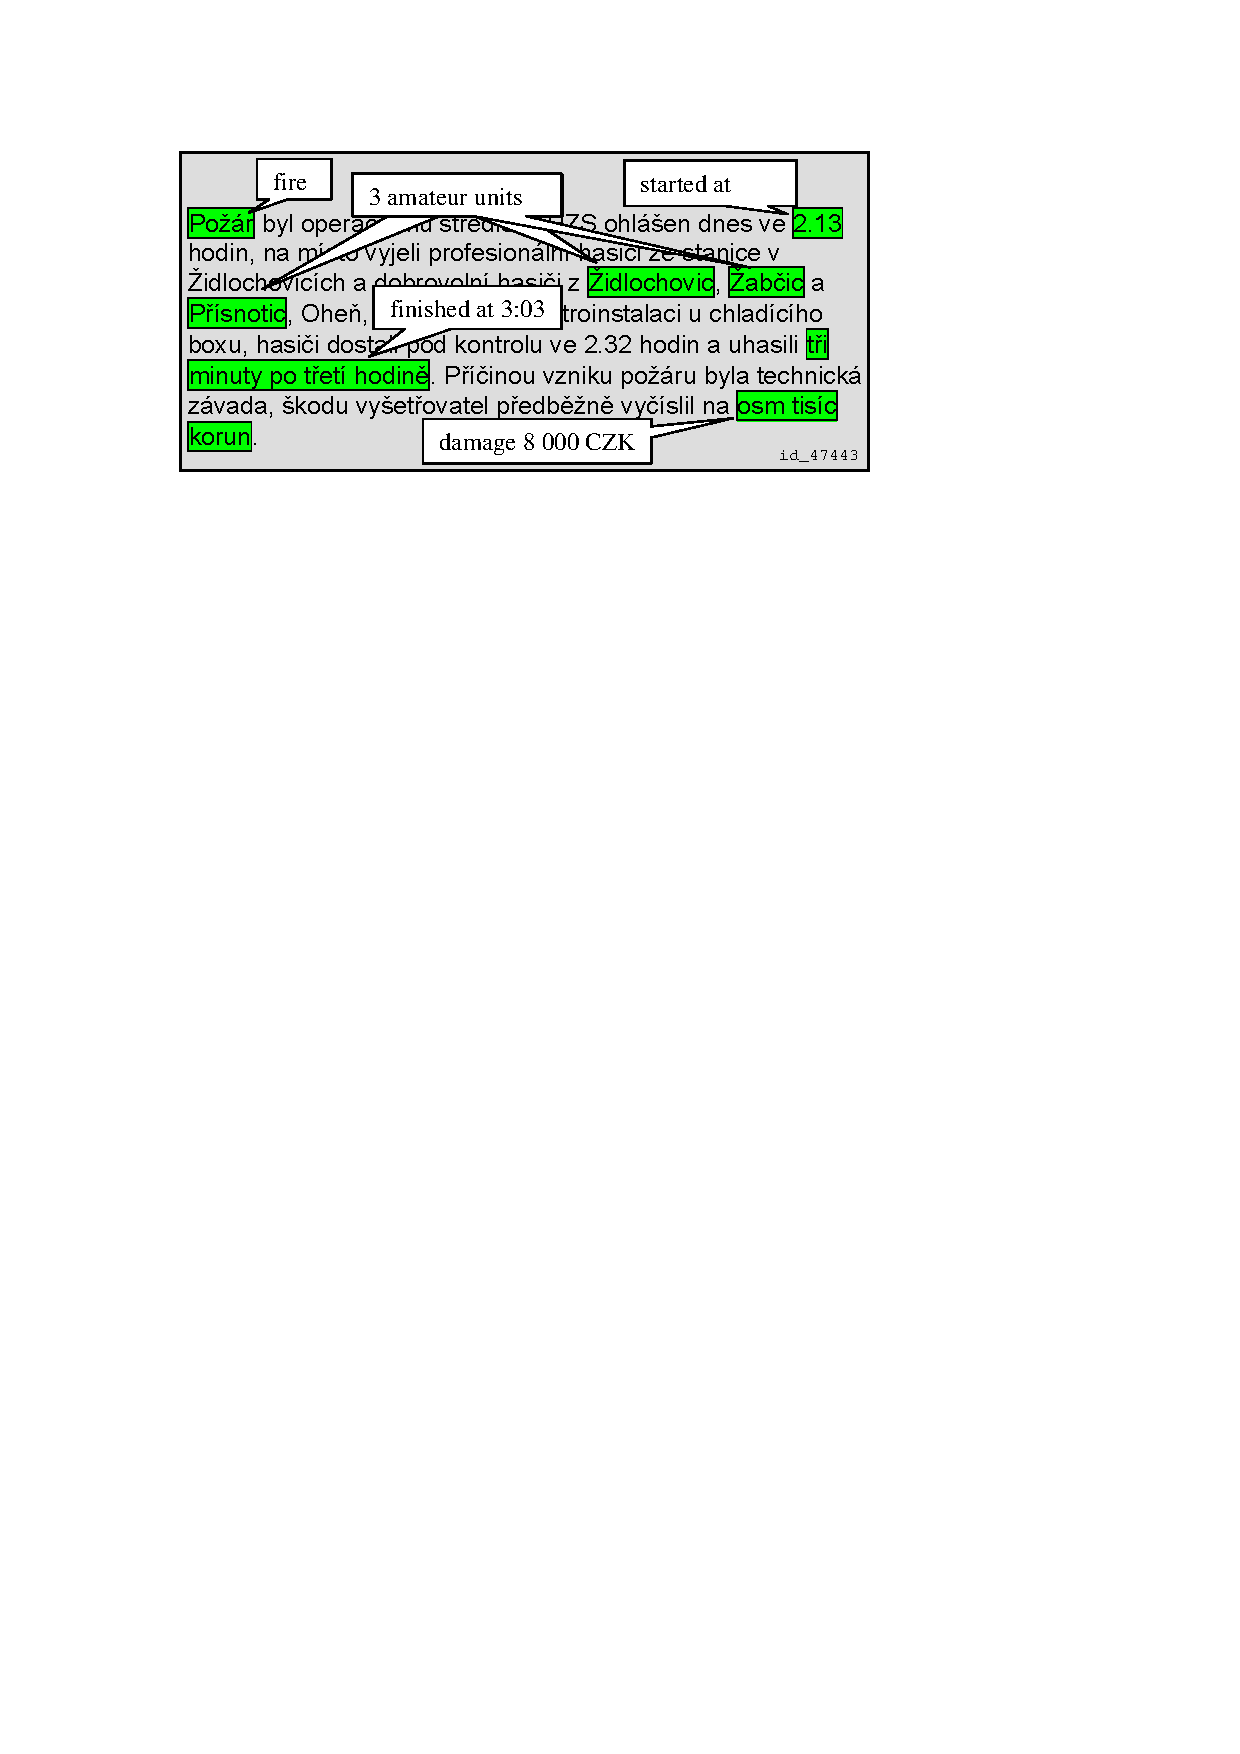
\includegraphics[width=0.75\hsize]{img/fireman_annotated}
	\end{center}	
	%\item The tools can also interpret such information in terms of a \alert{Semantic Web Ontology}.
\end{itemize}
\end{frame}

\subsection{Deep Language Parsing} 
\frame{\tableofcontents[currentsection, currentsubsection]}

\begin{frame}{Deep Language Parsing (Czech Example)}  
\begin{itemize}
	\item Linguistic tools perform automated linguistic analysis.
	\item Producing so called \emph{dependency trees}.
	%\begin{itemize}
		%\item Of course not 100\% accurete...
	%\end{itemize}
	\medskip	
	\begin{center}
	\framebox{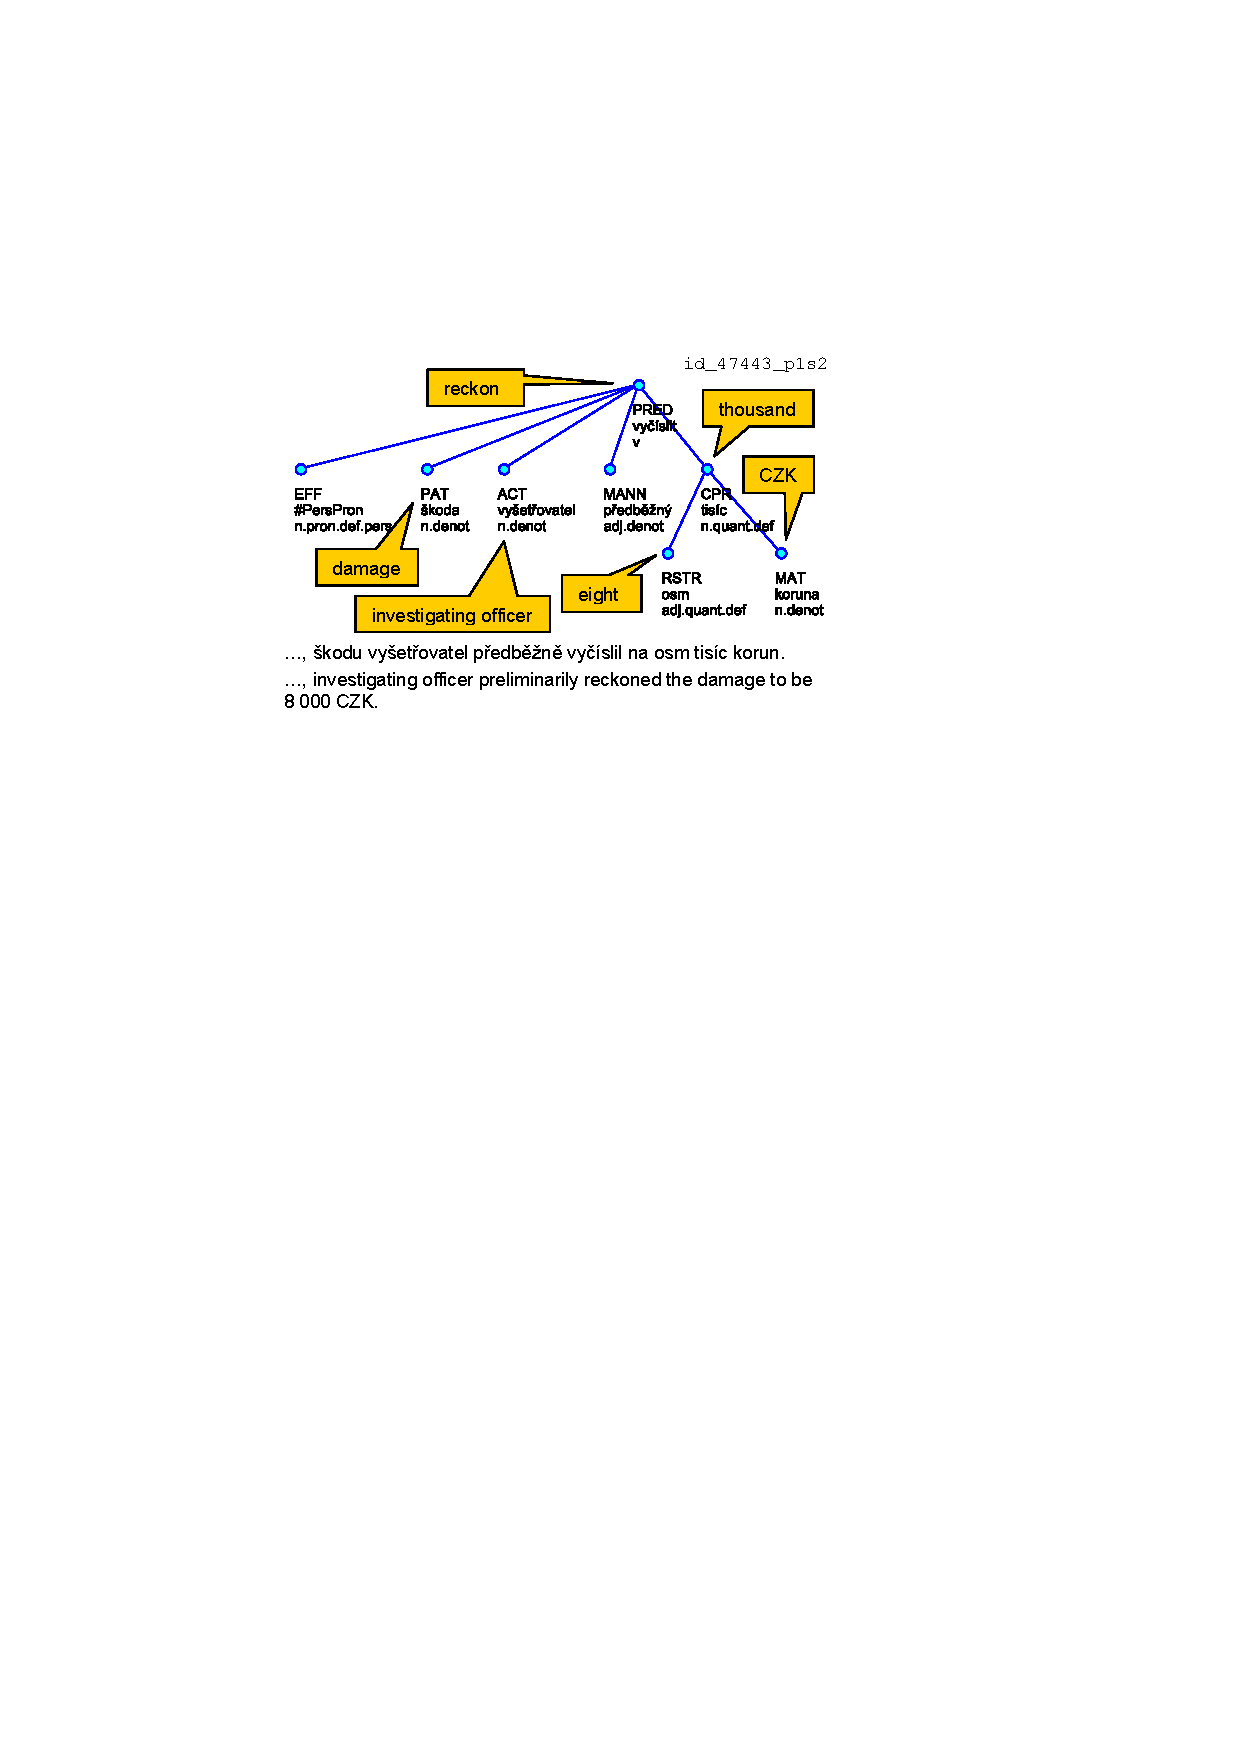
\includegraphics[width=0.63\hsize]{img/tree}}
	\end{center}	
	%\item The tools can also interpret such information in terms of a \alert{Semantic Web Ontology}.
\end{itemize}
\end{frame}

\begin{frame}{Layers of linguistic annotation in PDT}
\begin{columns}
\column{.5\textwidth}
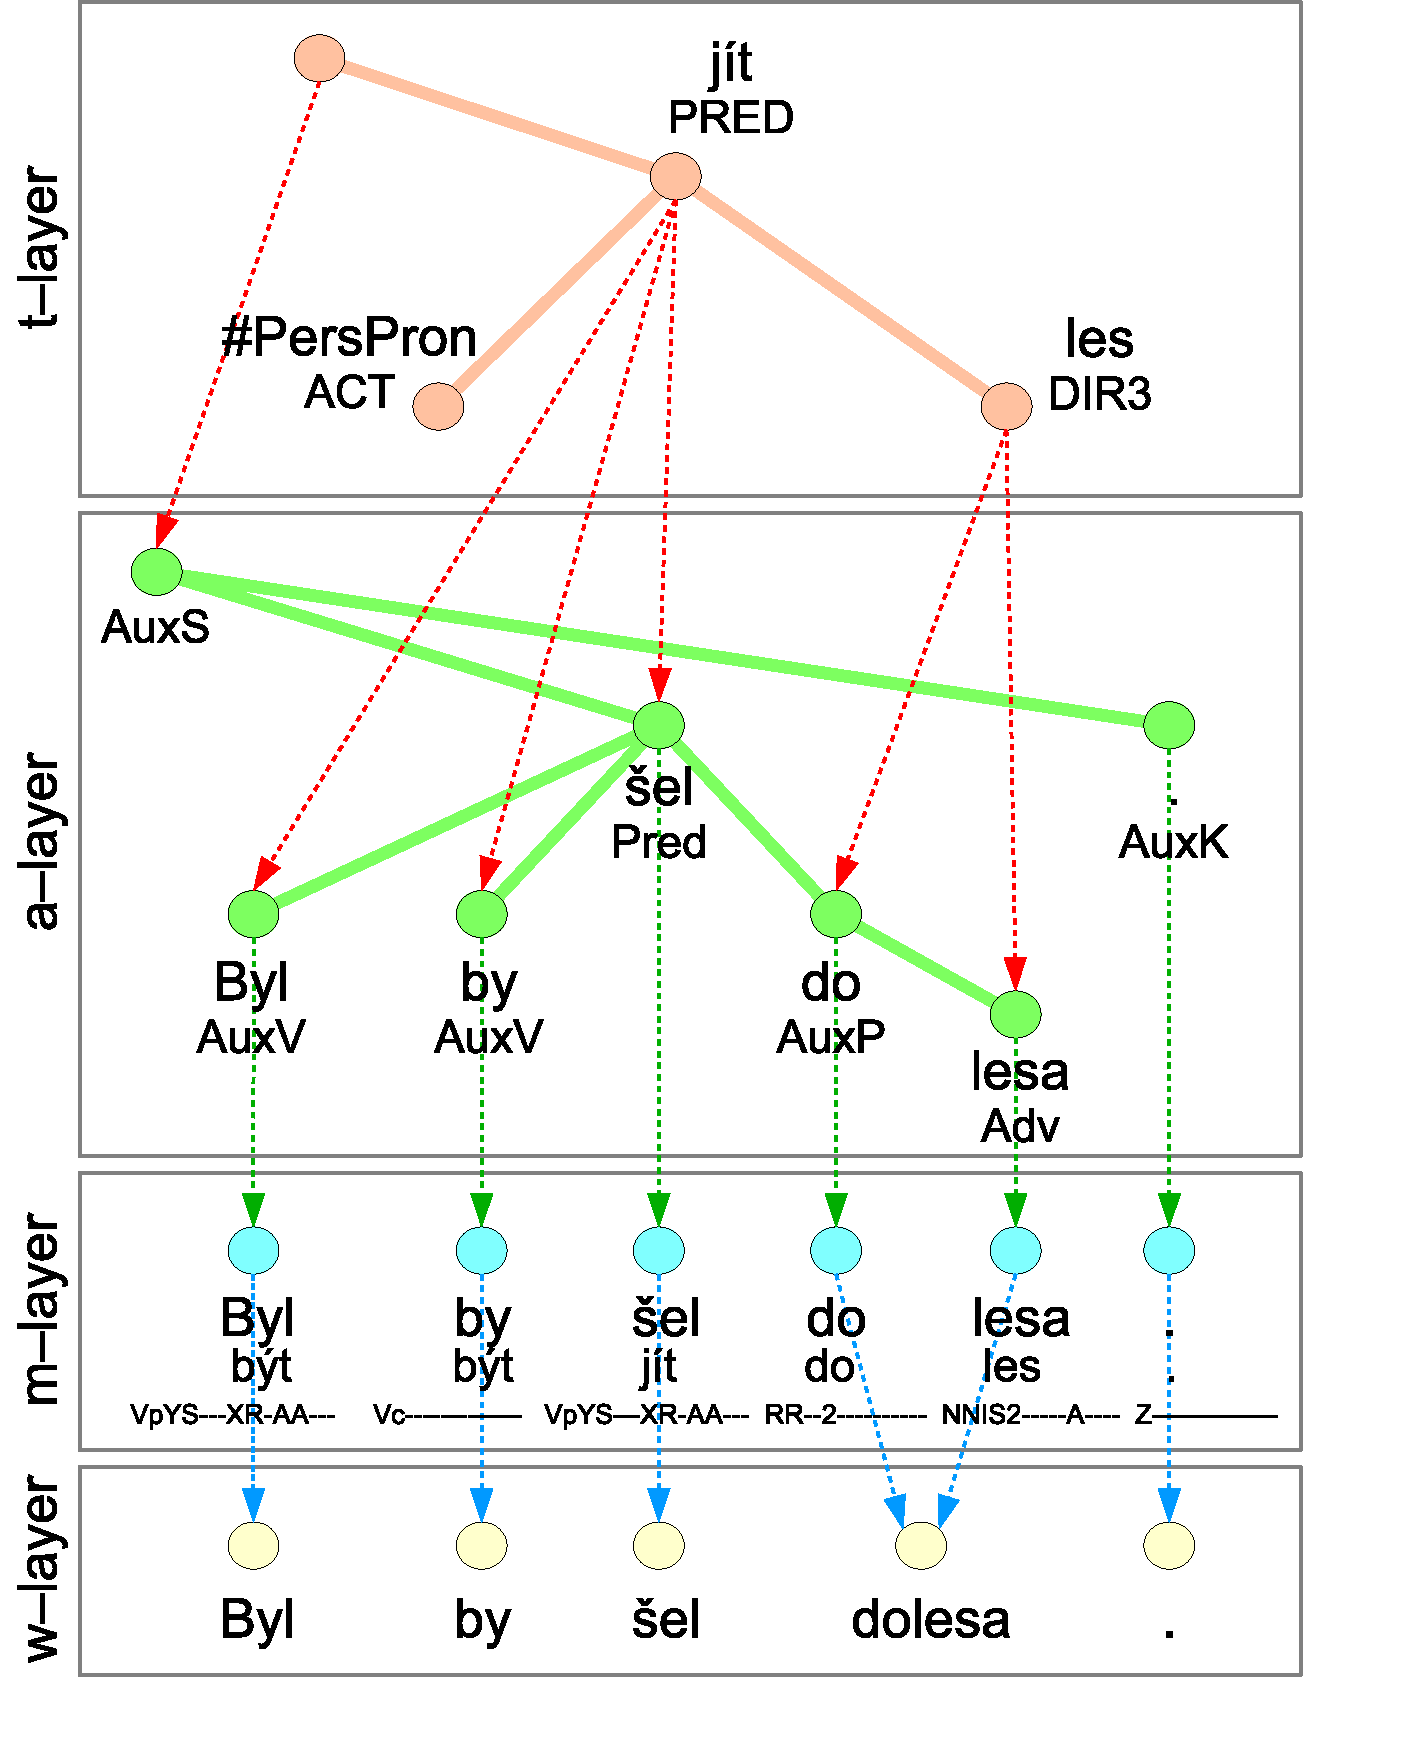
\includegraphics[height=0.9\vsize]{img/PDT_layers}
\column{.5\textwidth}
\begin{itemize}
	\item Tectogrammatical layer
	\item Analytical layer
	\item Morphological layer
\end{itemize}
\begin{itemize}
	\item PDT 2.0 on-line:\\\centerline{\scriptsize\url{http://ufal.mff.cuni.cz/pdt2.0/}} 
\end{itemize}
\vspace{2cm}
\emph{Sentence:}
\medskip
\\Byl by šel dolesa.
\\He-was would went toforest.
\end{columns}
\end{frame}


\subsection{Inductive Logic Programming} 
\frame{\tableofcontents[currentsection, currentsubsection]}

\begin{frame}{Inductive Logic Programming}
\begin{itemize}
	\item Learning examples $E=P\cup N$ (Positive and Negative)	
	\begin{itemize}
		\item E.g. relevant and irrelevant pieces of text w.r.t. particular extraction task
	\end{itemize}	
	\item Background knowledge $B$
	\begin{itemize}
		\item E.g. linguistic structure connecting individual words
	\end{itemize}	
	\item ILP task: To find logical program or hypothesis $H$ such that all positive examples are covered and none negative
$$
(\forall e\in P)(B\cup H\models e) \ \ \&\  \ (\forall n\in N)(B\cup H\not\models n).
$$
	\begin{itemize}
		\item E.g. to find common pattern (in the linguistic structure) present around every relevant piece of text and none irrelevant.
	\end{itemize}	
\end{itemize}
\end{frame}


\subsection{Organization of this Presentation} 
\frame{\tableofcontents[currentsection, currentsubsection]}

\begin{frame}{Four Main Topics}

\begin{itemize}
	\item \themetext[colorManual]{Manual Design of Extraction Rules}
	\item \themetext[colorLearning]{Induction of Extraction Rules}
	\item \themetext[colorShareable]{Shareable Extraction Ontologies}
	\item \themetext[colorFuzzy]{Fuzzy ILP Document Classification}
\end{itemize}

\end{frame}


\themecolor{\colorManual}
\begin{frame}{Manual Design of Extraction Rules}
Slides about the topic \emph{Manual Design of Extraction Rules} will have \themetext[colorManual]{brown }  headline background.
\end{frame}

\themecolor{\colorLearning}
\begin{frame}{Induction of Extraction Rules}
Slides about the topic \emph{Induction of Extraction Rules} will have \themetext[colorLearning]{green }  headline background.
\end{frame}

\themecolor{\colorShareable}
\begin{frame}{Shareable Extraction Ontologies}
Slides about the topic \emph{Shareable Extraction Ontologies} will have \themetext[colorShareable]{cyan }  headline background.
\end{frame}

\themecolor{\colorFuzzy}
\begin{frame}{Fuzzy ILP Document Classification}
Slides about the topic \emph{Fuzzy ILP Document Classification} will have \themetext[colorFuzzy]{magenta }  headline background.
\end{frame}

\resetcolor
\begin{frame}{Ordinary}
\end{frame}


\section{Contents}
\subsection{Manual Design of Extraction Rules}
\themecolor{\colorManual}
\frame{\frametitle{Manual Design of Extraction Rules} \tableofcontents[currentsection, currentsubsection]}


\begin{frame}[plain]
\begin{columns}
\column{.55\textwidth}
%\centerline{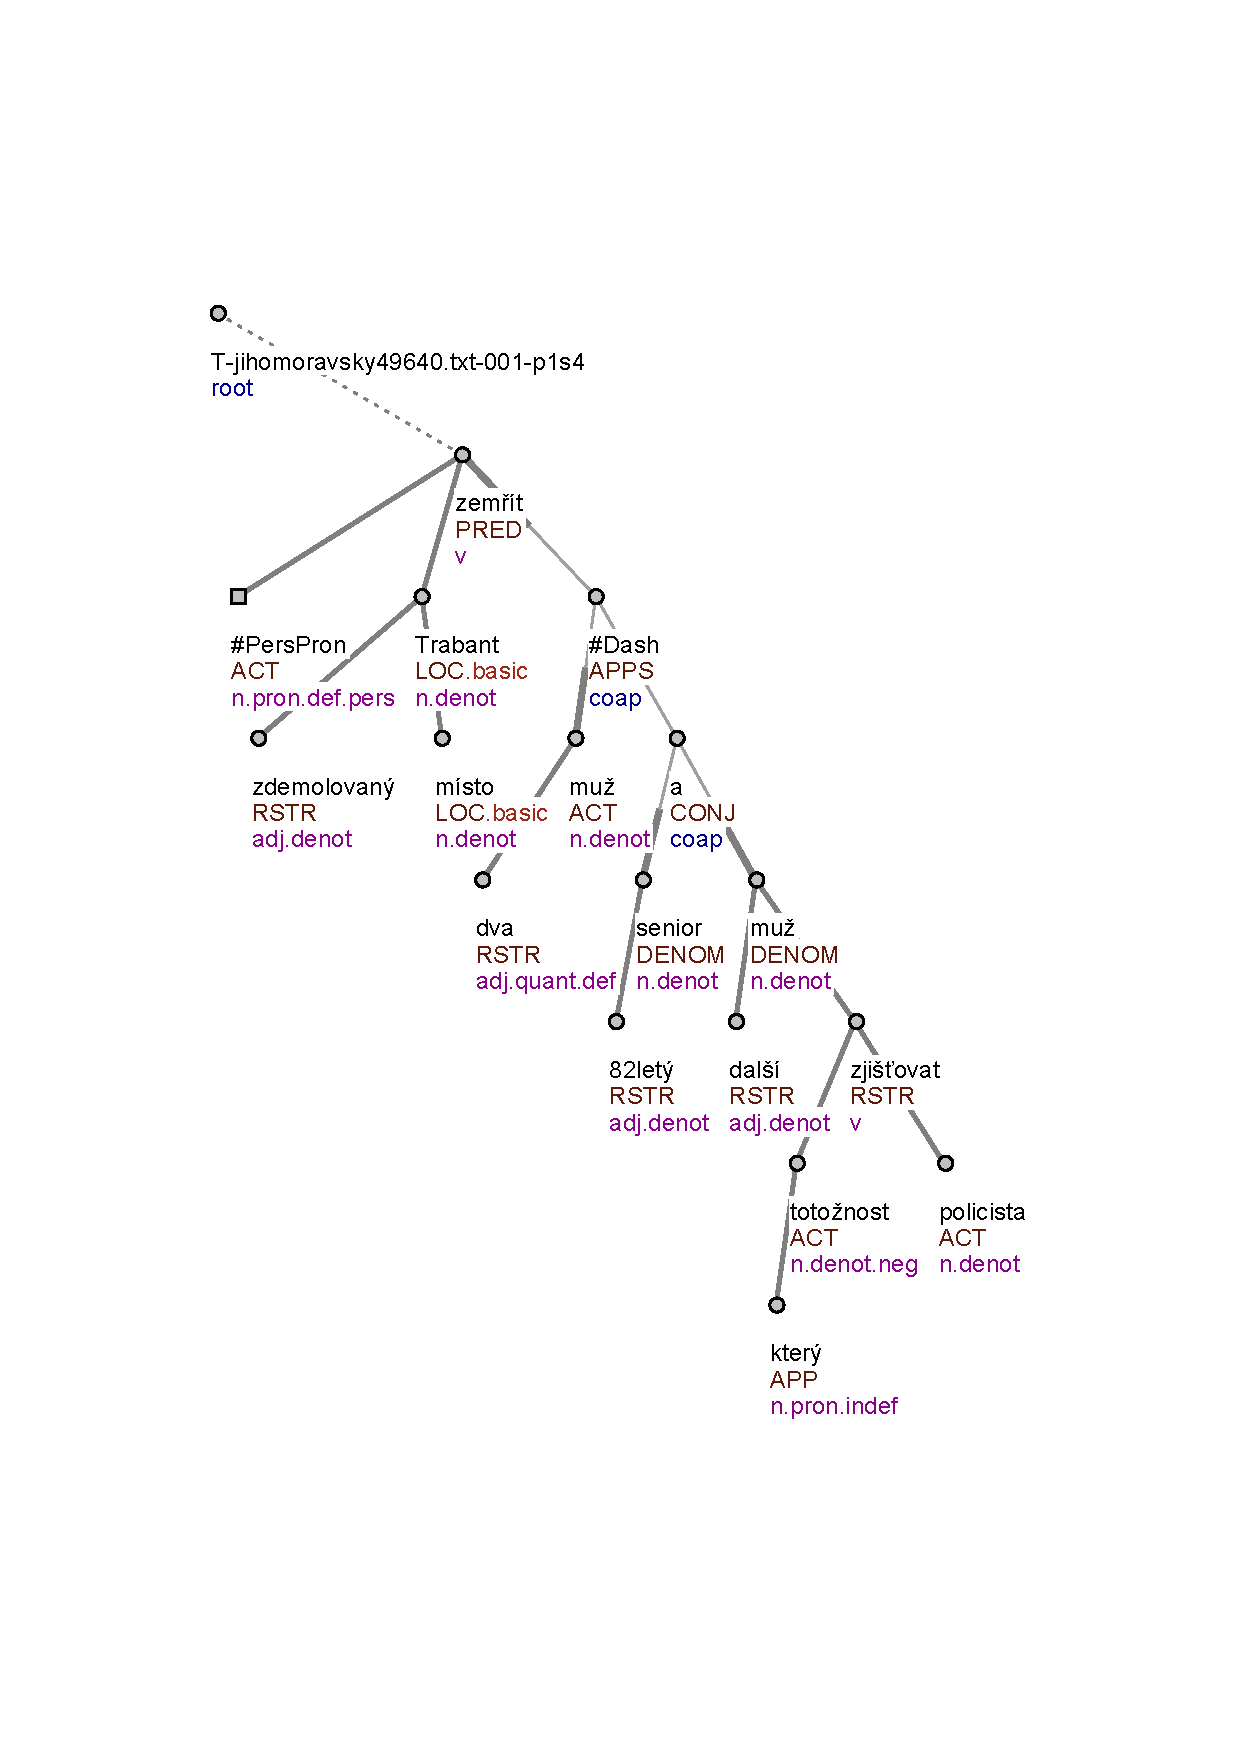
\includegraphics[height=1.1\vsize,width=\hsize]{img/TectogramaticalTree}}
\centerline{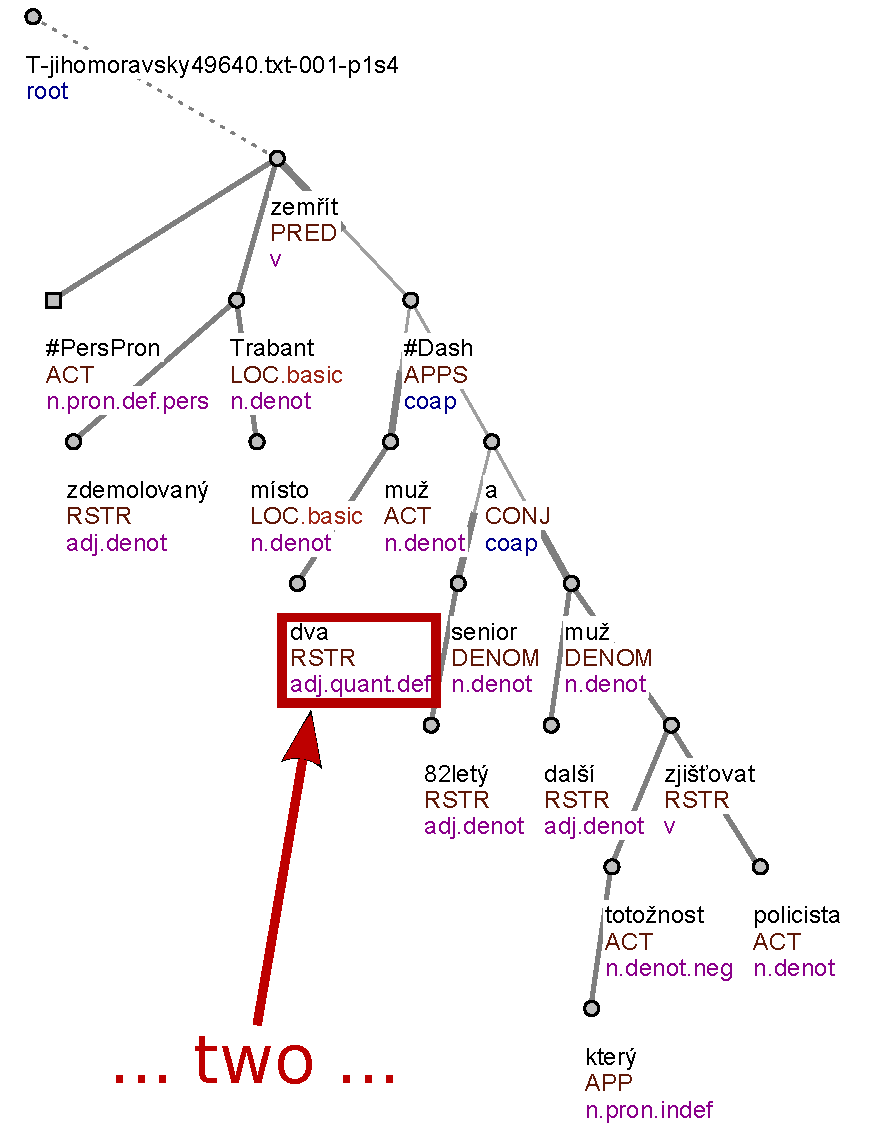
\includegraphics[height=0.95\vsize]{img/Two_Tree}}
\column{.45\textwidth}
\begin{itemize}
	\item How to extract the information about \alert{two dead} people?
\bigskip
	\item \emph{Sentence:}
\medskip
{\small
\\Ve zdemolovaném trabantu na místě \alert{zemřeli dva muži} -- 82letý senior a další muž, jehož totožnost zjišťují policisté.
\medskip
\\\alert{Two men died} on the spot in demolished trabant -- \dots }
\end{itemize}
\vspace{2cm}
\end{columns}
\end{frame}




\begin{frame}{Extraction rules -- Netgraph queries}
\begin{center}
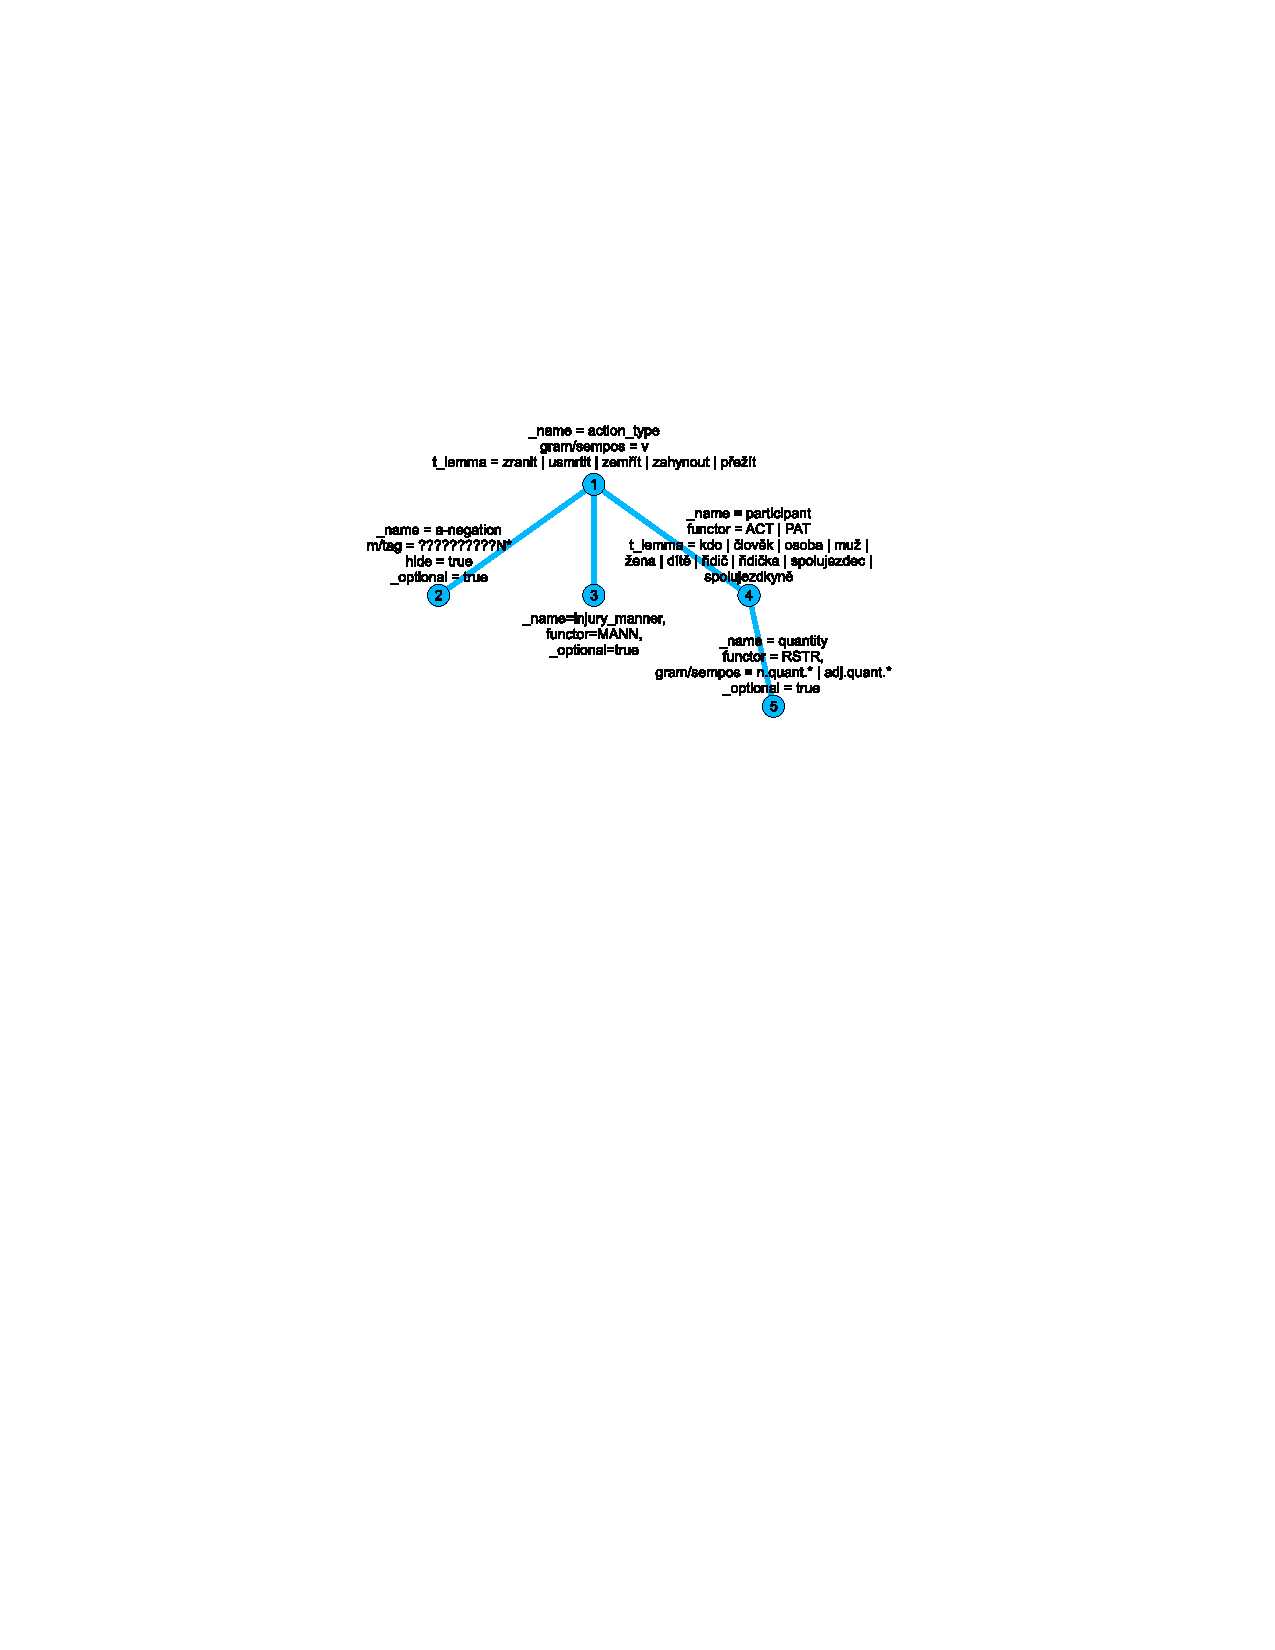
\includegraphics[height=0.6\vsize]{img/extract_patern}
\end{center}
\begin{itemize}
	\item Tree patterns on \alert{shape} and \alert{nodes} (on node attributes).
	\item Evaluation gives \alert{actual matches} of particular nodes.
	\item \alert{Names} of nodes allow use of references.
\end{itemize}
\end{frame}


\begin{frame}{Raw data extraction output}
%\begin{center}
\centerline{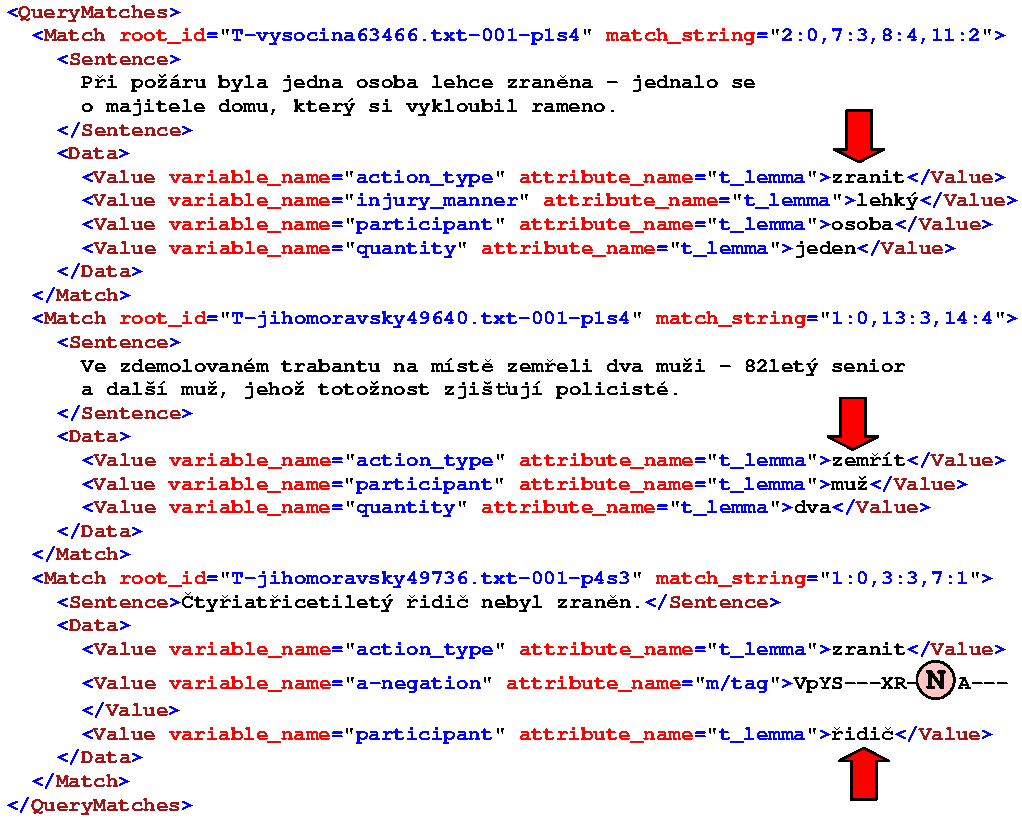
\includegraphics[height=0.75\vsize]{img/OutputQueryMatches}}
%\end{center}

{\scriptsize
\textbf{SELECT} \alert{action\_type}.t\_lemma, \alert{a-negation}.m\/tag, 
\alert{injury\_manner}.t\_lemma, \alert{participant}.t\_lemma,
\alert{quantity}.t\_lemma \textbf{FROM} \emph{***extraction rule***} 
}
\end{frame}

\begin{frame}{Extraction rules -- Environment Protection Use Case}
\begin{center}
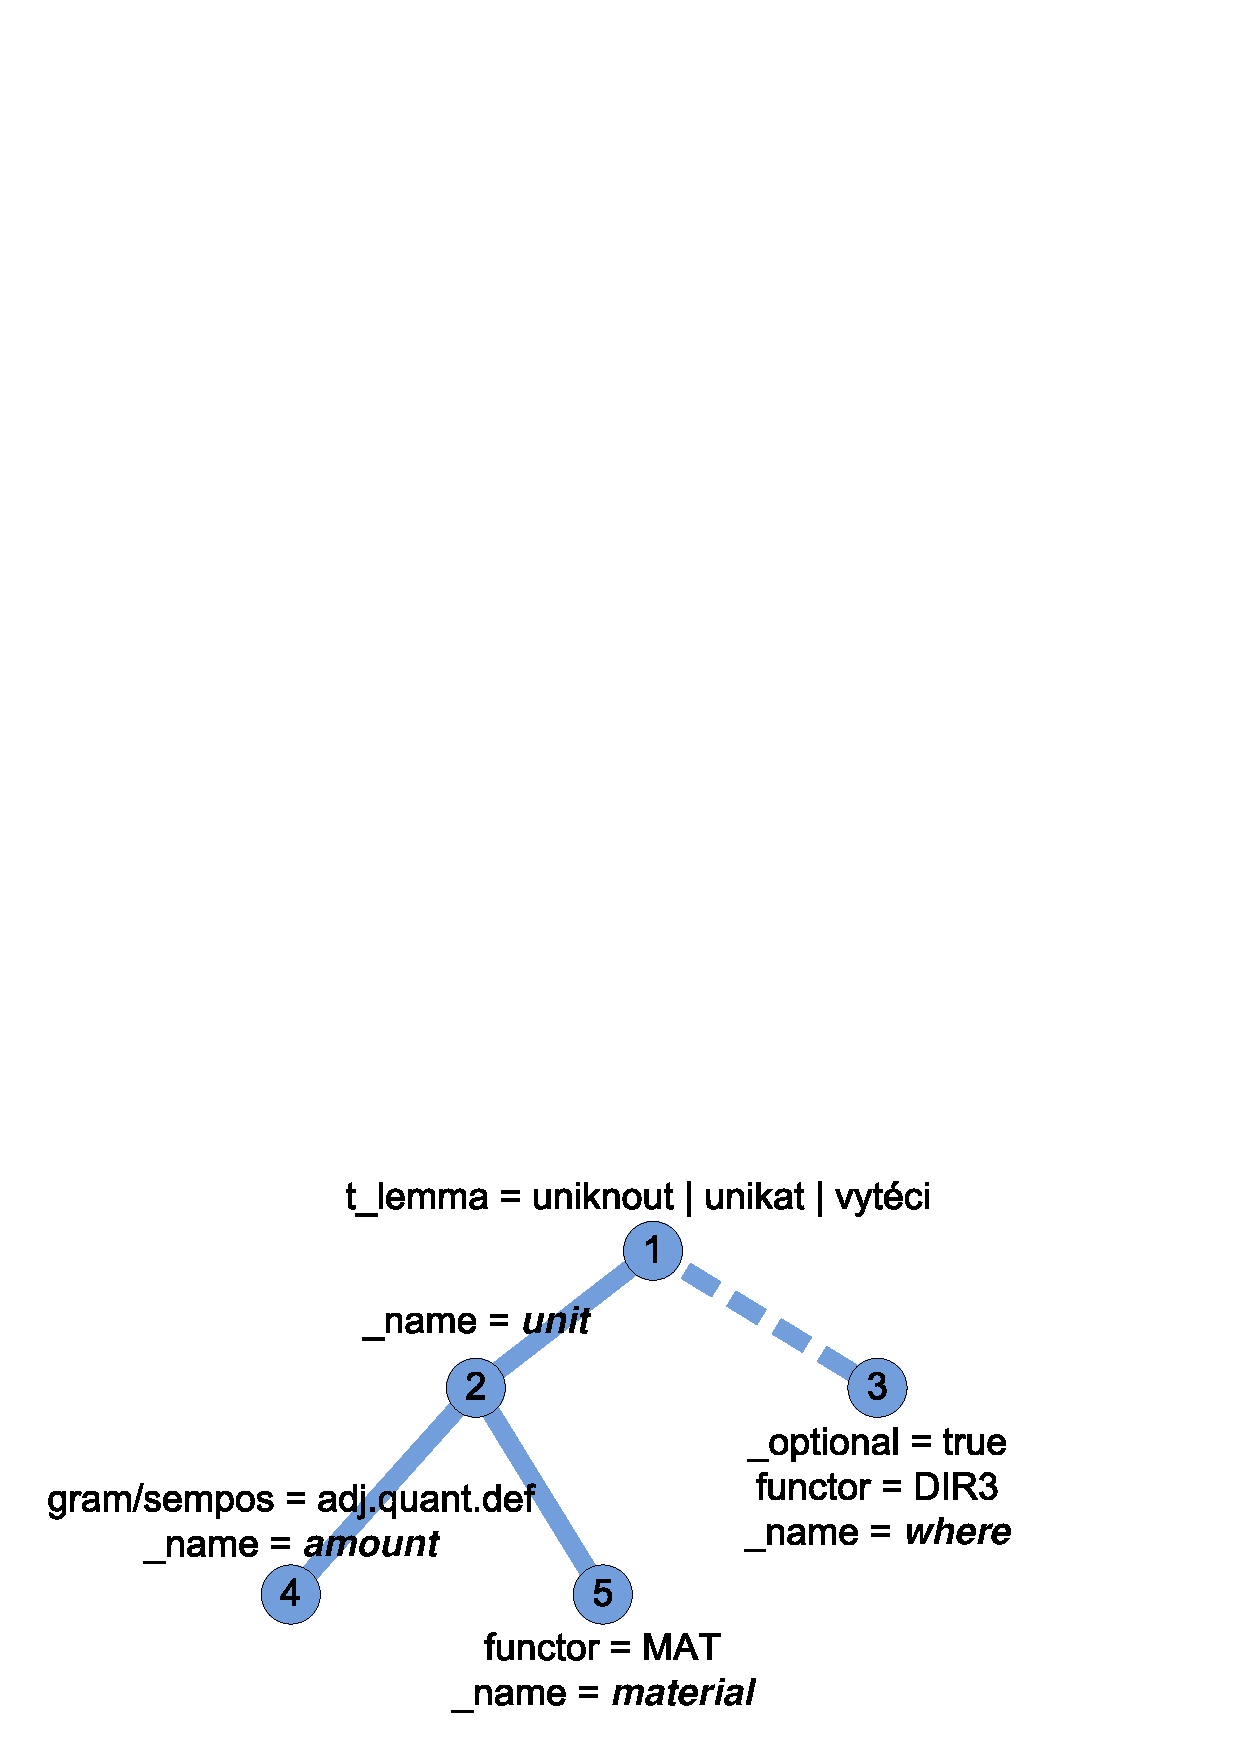
\includegraphics[height=0.5\vsize]{img/eenv_extr_rule}
\end{center}
%\begin{itemize}
%	\item Tree patterns on \alert{shape} and \alert{nodes} (on node attributes).
%	\item Evaluation gives \alert{actual matches} of particular nodes.
%	\item \alert{Names} of nodes allow use of references.
%\end{itemize}
\end{frame}



\begin{frame}{Matching Tree}
%\begin{center}
\centerline{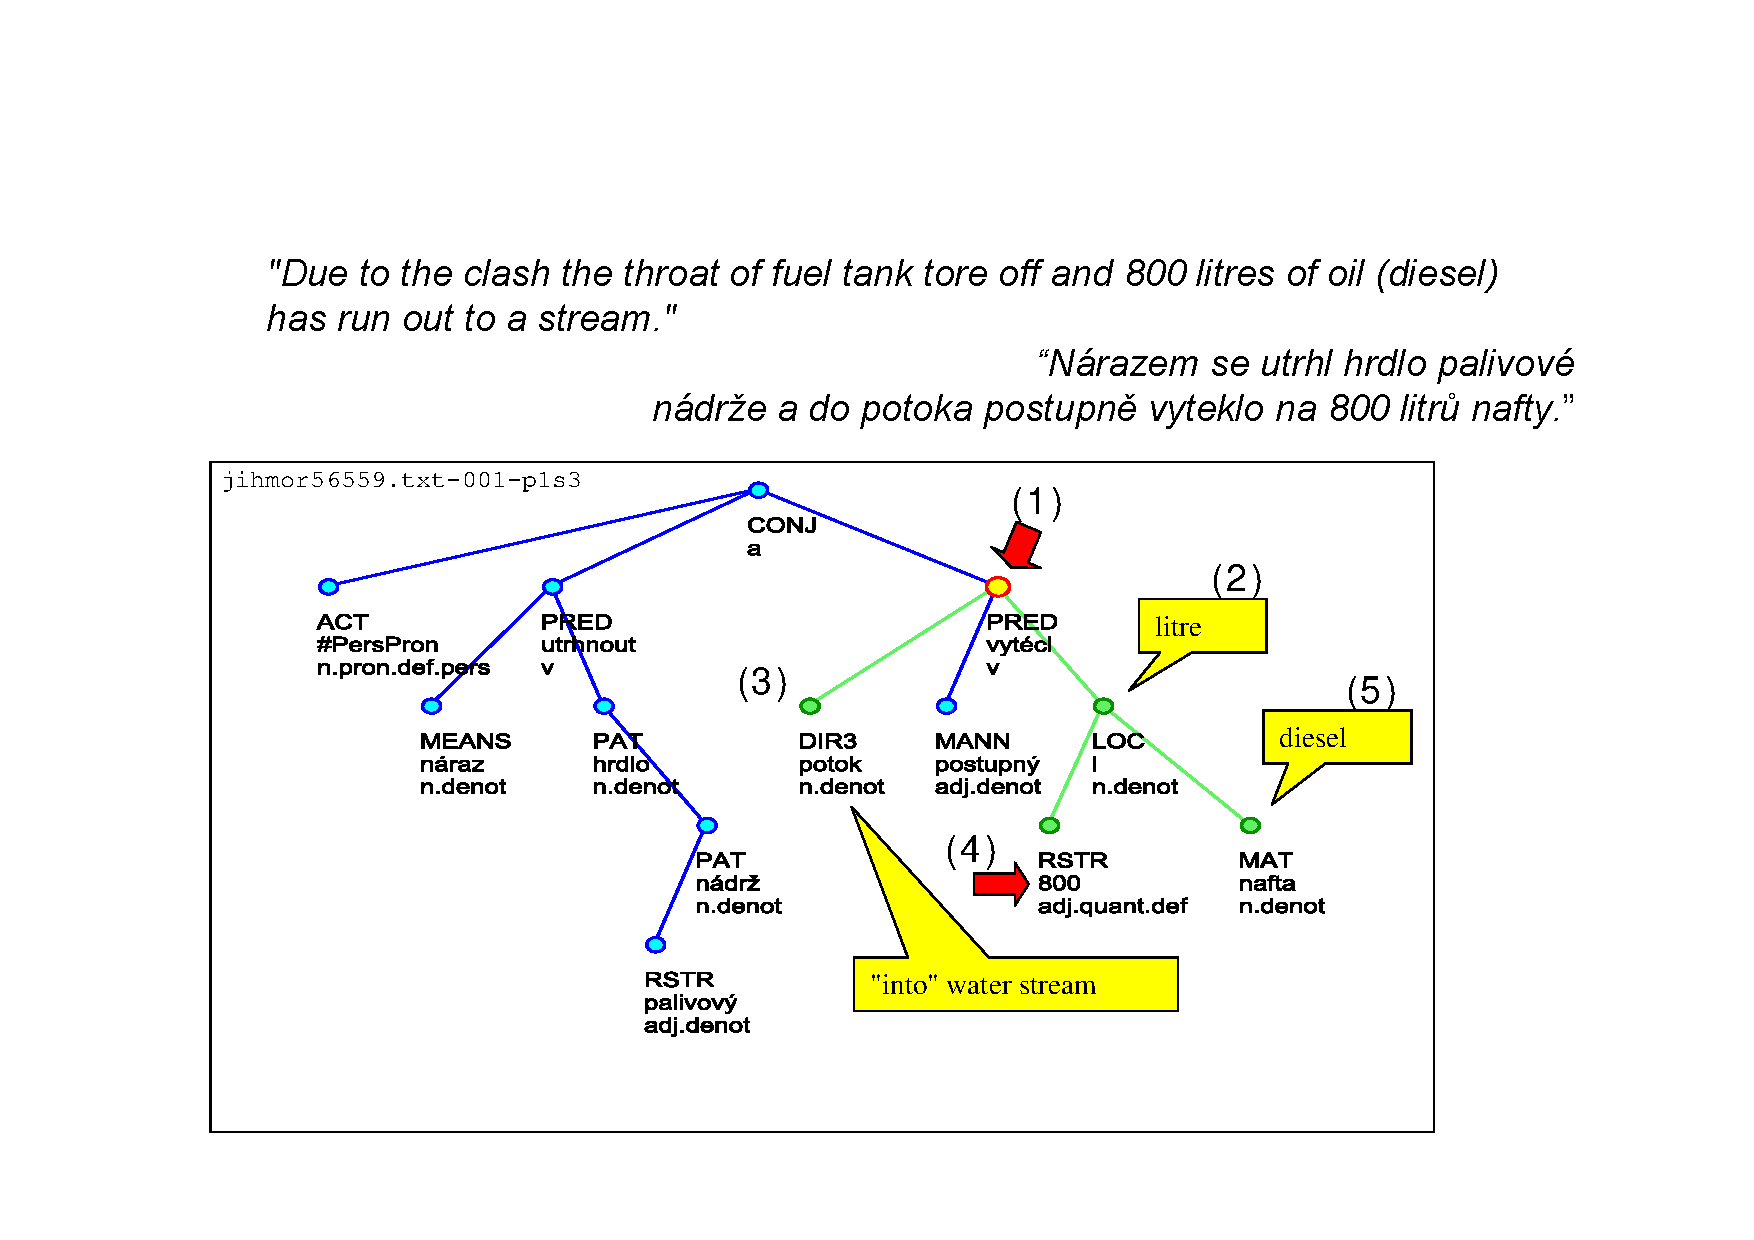
\includegraphics[height=1.15\vsize, angle=-90]{img/eenv_tree}}
%\end{center}
%{\scriptsize
%\textbf{SELECT} \alert{action\_type}.t\_lemma, \alert{a-negation}.m\/tag, 
%\alert{injury\_manner}.t\_lemma, \alert{participant}.t\_lemma,
%\alert{quantity}.t\_lemma \textbf{FROM} \emph{***extraction rule***} 
%}
\end{frame}


\begin{frame}{Raw data extraction output}
%\begin{center}
\centerline{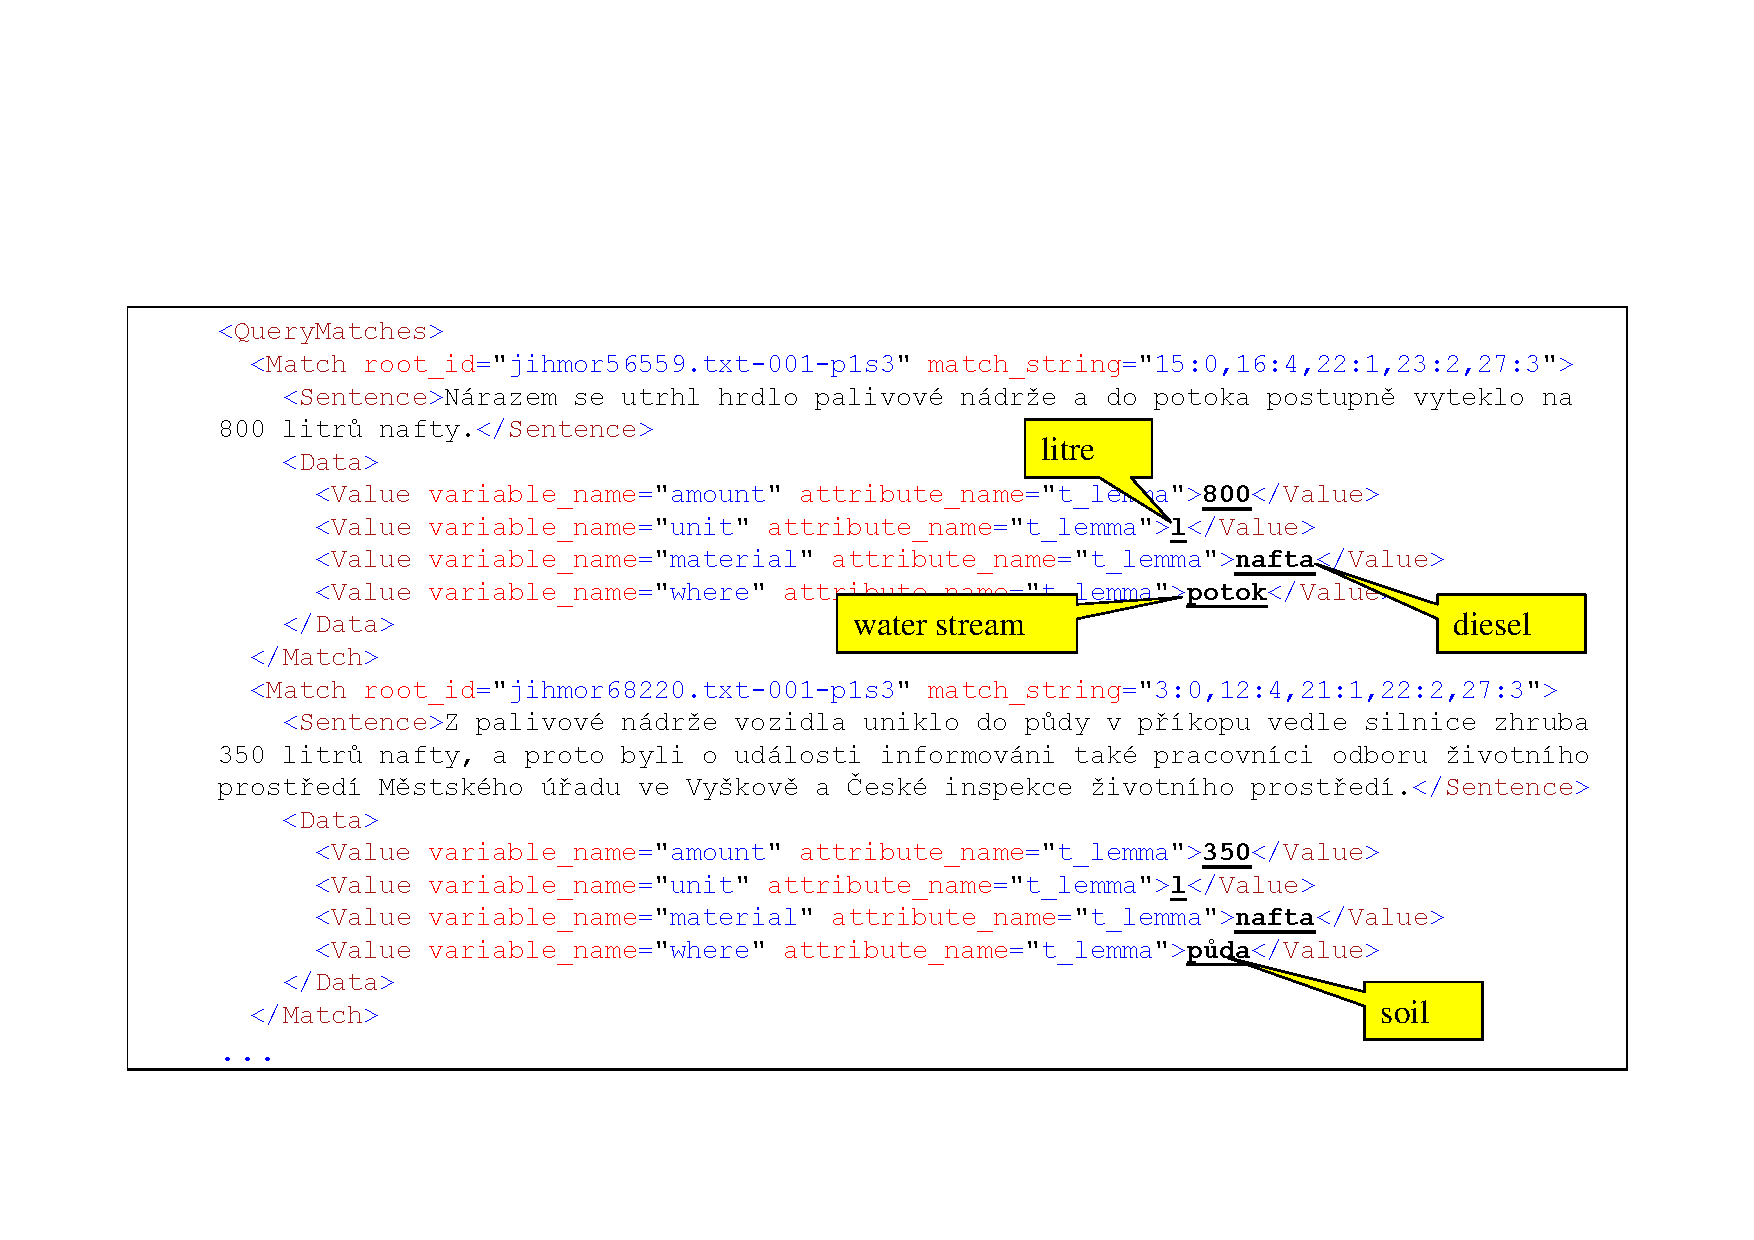
\includegraphics[height=1.25\vsize, angle=-90]{img/eenv_results}}
%\end{center}
{\scriptsize
\medskip
\textbf{SELECT} \alert{amount}.t\_lemma, \alert{unit}.t\_lemma, 
\alert{material}.t\_lemma, \alert{where}.t\_lemma
\\ \textbf{FROM} \emph{***extraction rule***} 
}
\end{frame}



\begin{frame}{Design of extraction rules -- iterative process}
\begin{center}
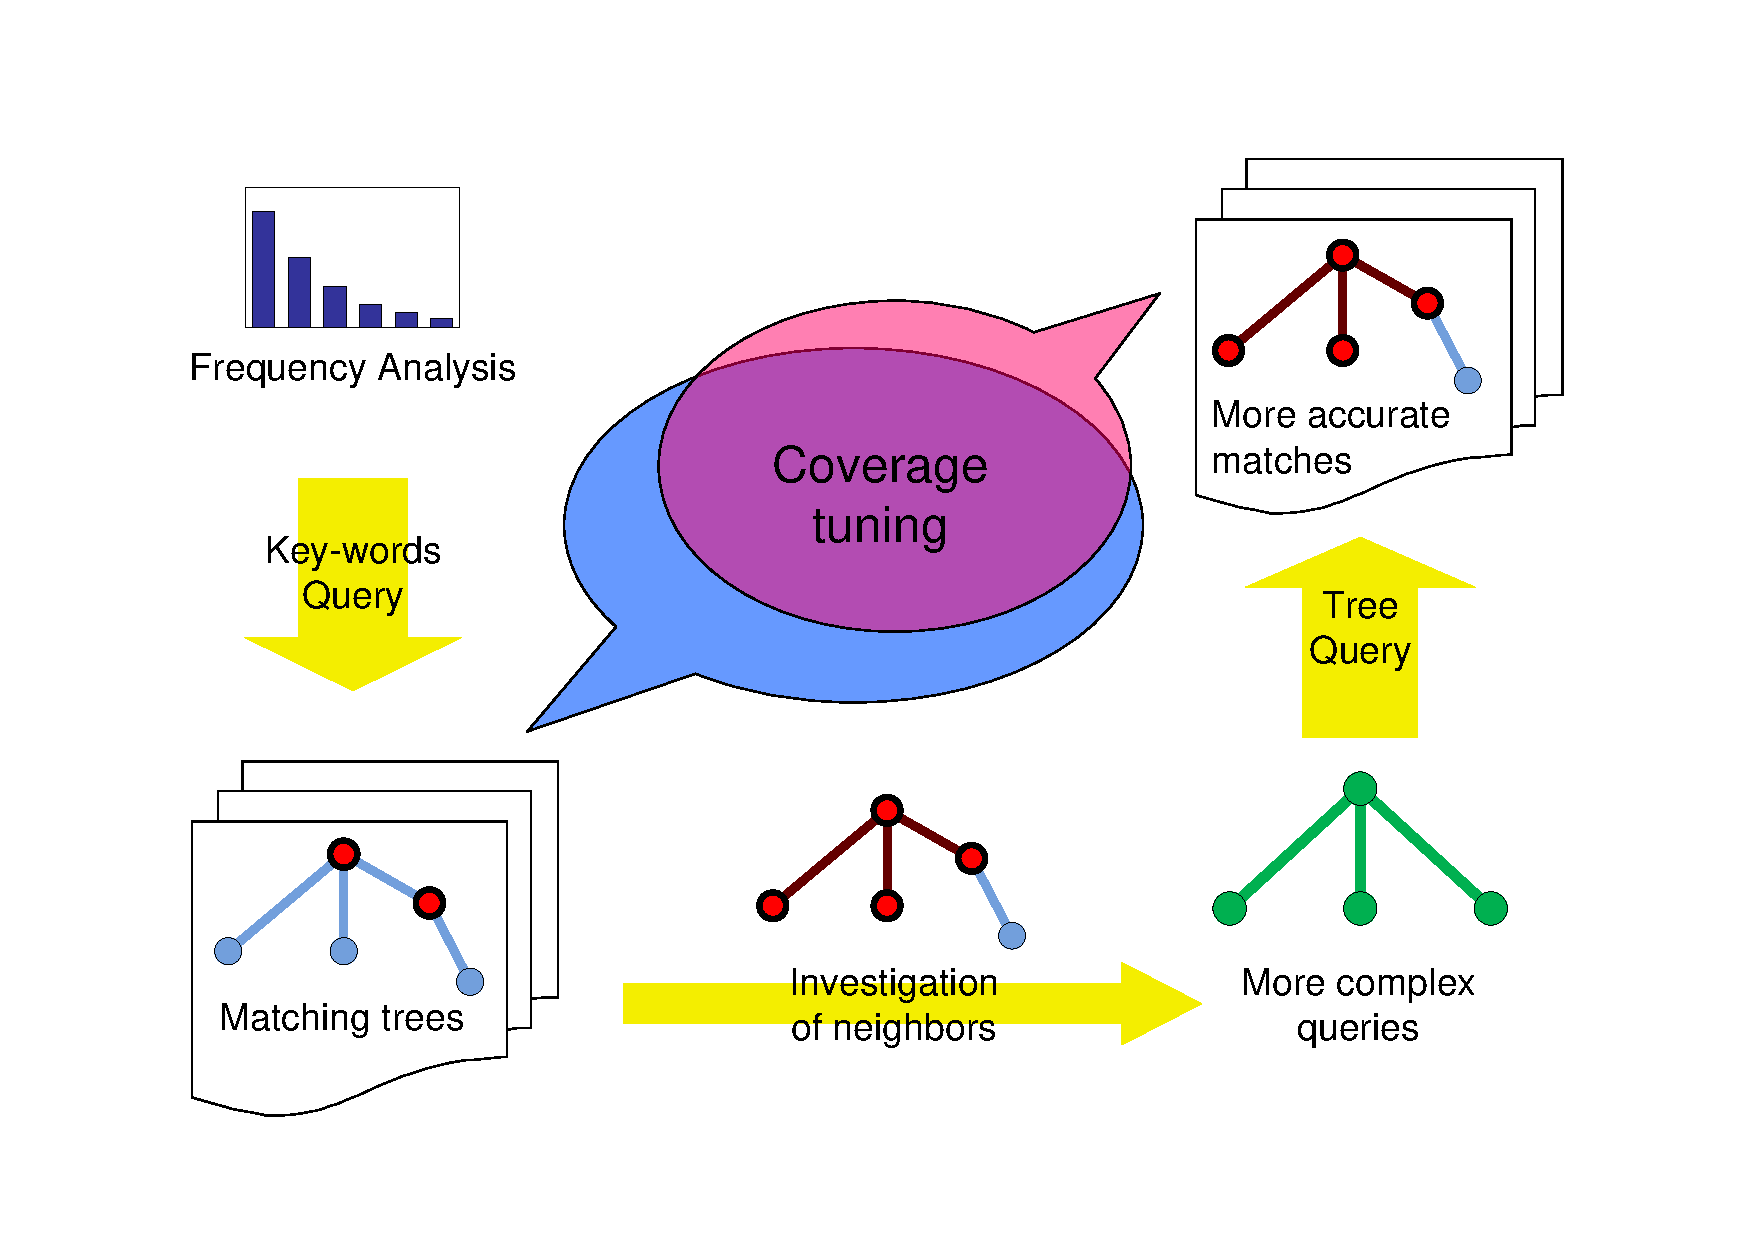
\includegraphics[height=0.8\vsize, angle=-90]{img/coverge_tuning}
\end{center}
\begin{enumerate}
	\item \alert{Frequency analysis} $\rightarrow$ representative key-words.
	\item Investigating of matching trees $\rightarrow$ \alert{tuning} of tree query.
	\item \alert{Complexity} of the query $\cong$ complexity of extracted data.
\end{enumerate}
\end{frame}


\begin{frame}{Semantic interpretation of extraction rules}
\begin{center}
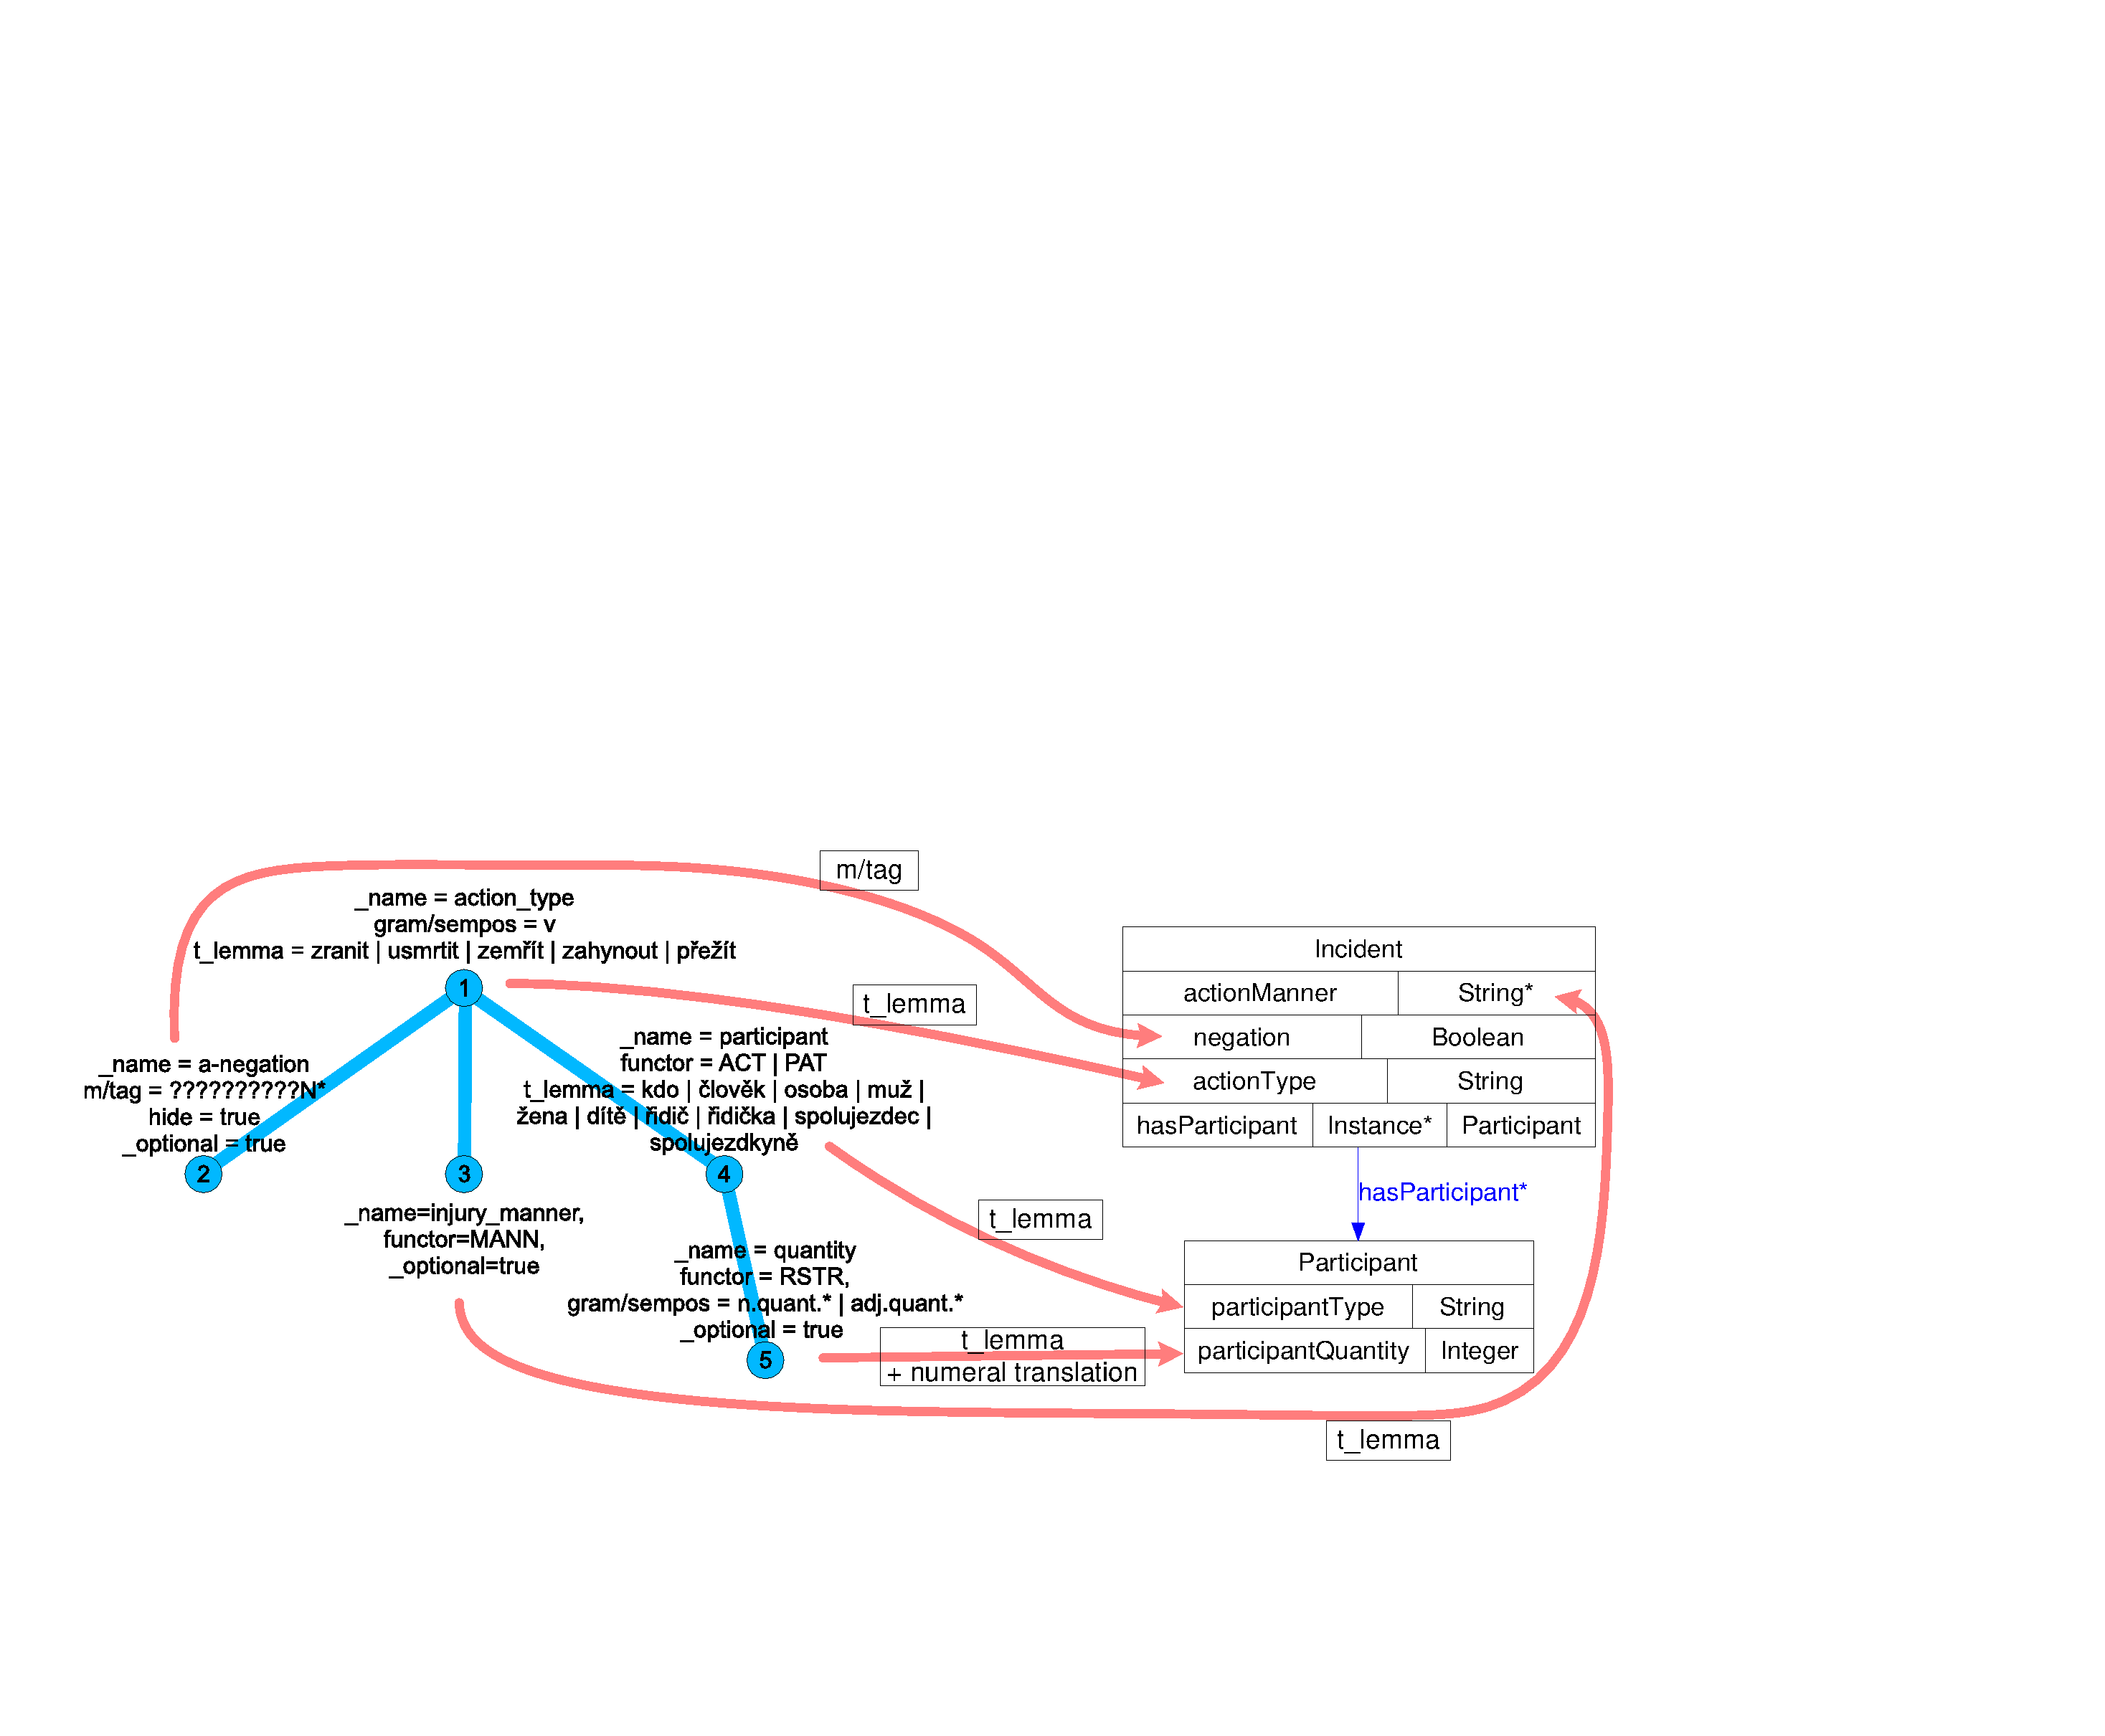
\includegraphics[width=0.55\vsize, angle=-90]{img/semantic_interpretation}
\end{center}
\begin{itemize}
	\item Determines how particular values of attributes are used.
	\item Gives semantics to extraction rule.
	\item Gives semantics to extracted data.
	\item Only proposal
\end{itemize}
\end{frame}


\subsection{Induction of Extraction Rules}
\themecolor{\colorLearning}
\frame{\frametitle{Induction of Extraction Rules} \tableofcontents[currentsection, currentsubsection]}

\begin{frame}{Integration of ILP in our extraction process}
\begin{center}
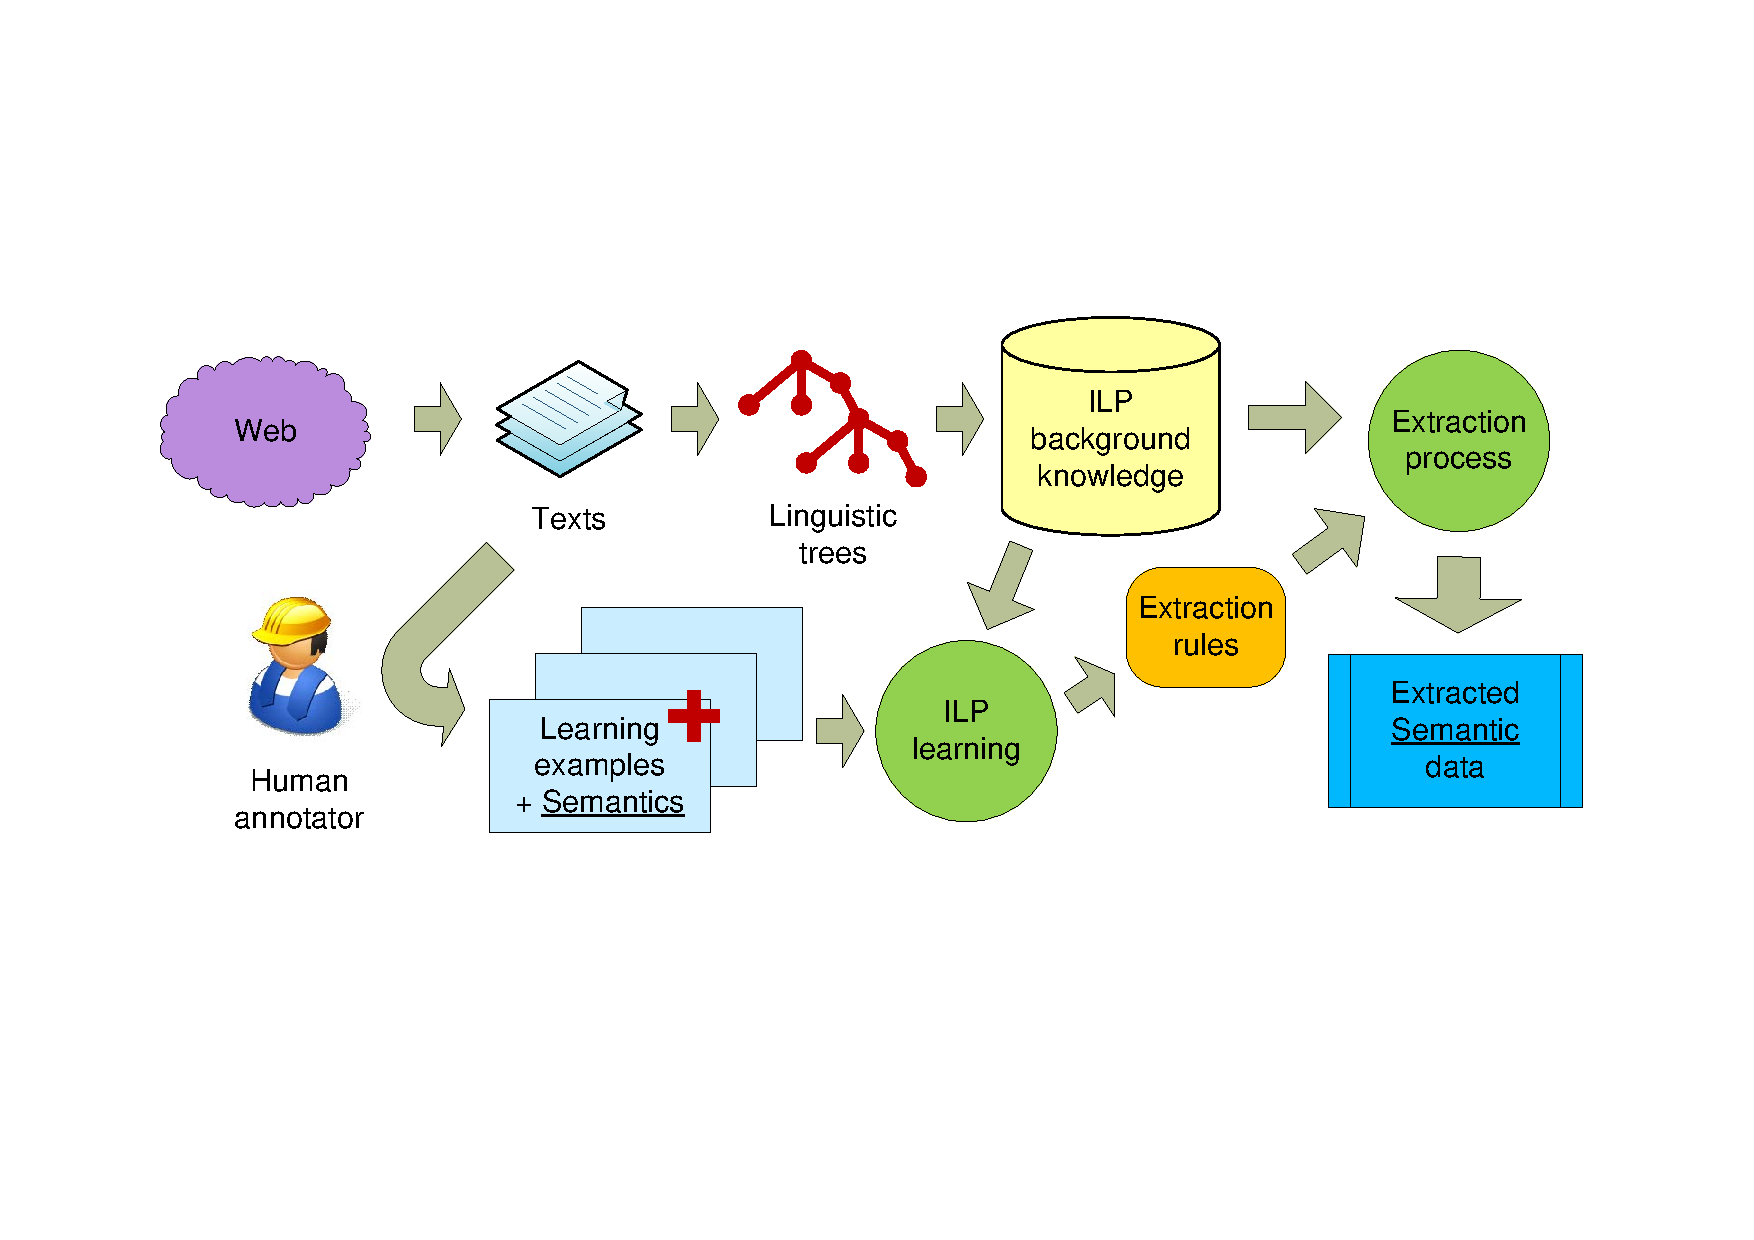
\includegraphics[width=0.45\vsize, angle=-90]{img/ILP_IE_process}
\end{center}
\begin{itemize}
	\item Main point: transformation of trees to \alert{logic representation}. 
	\item Human annotator does \alert{not} need to be a linguistic \alert{expert}.
\end{itemize}
\end{frame}

\begin{frame}{Logic representation of linguistic trees}
\begin{columns}
\column{\textwidth}
\centerline{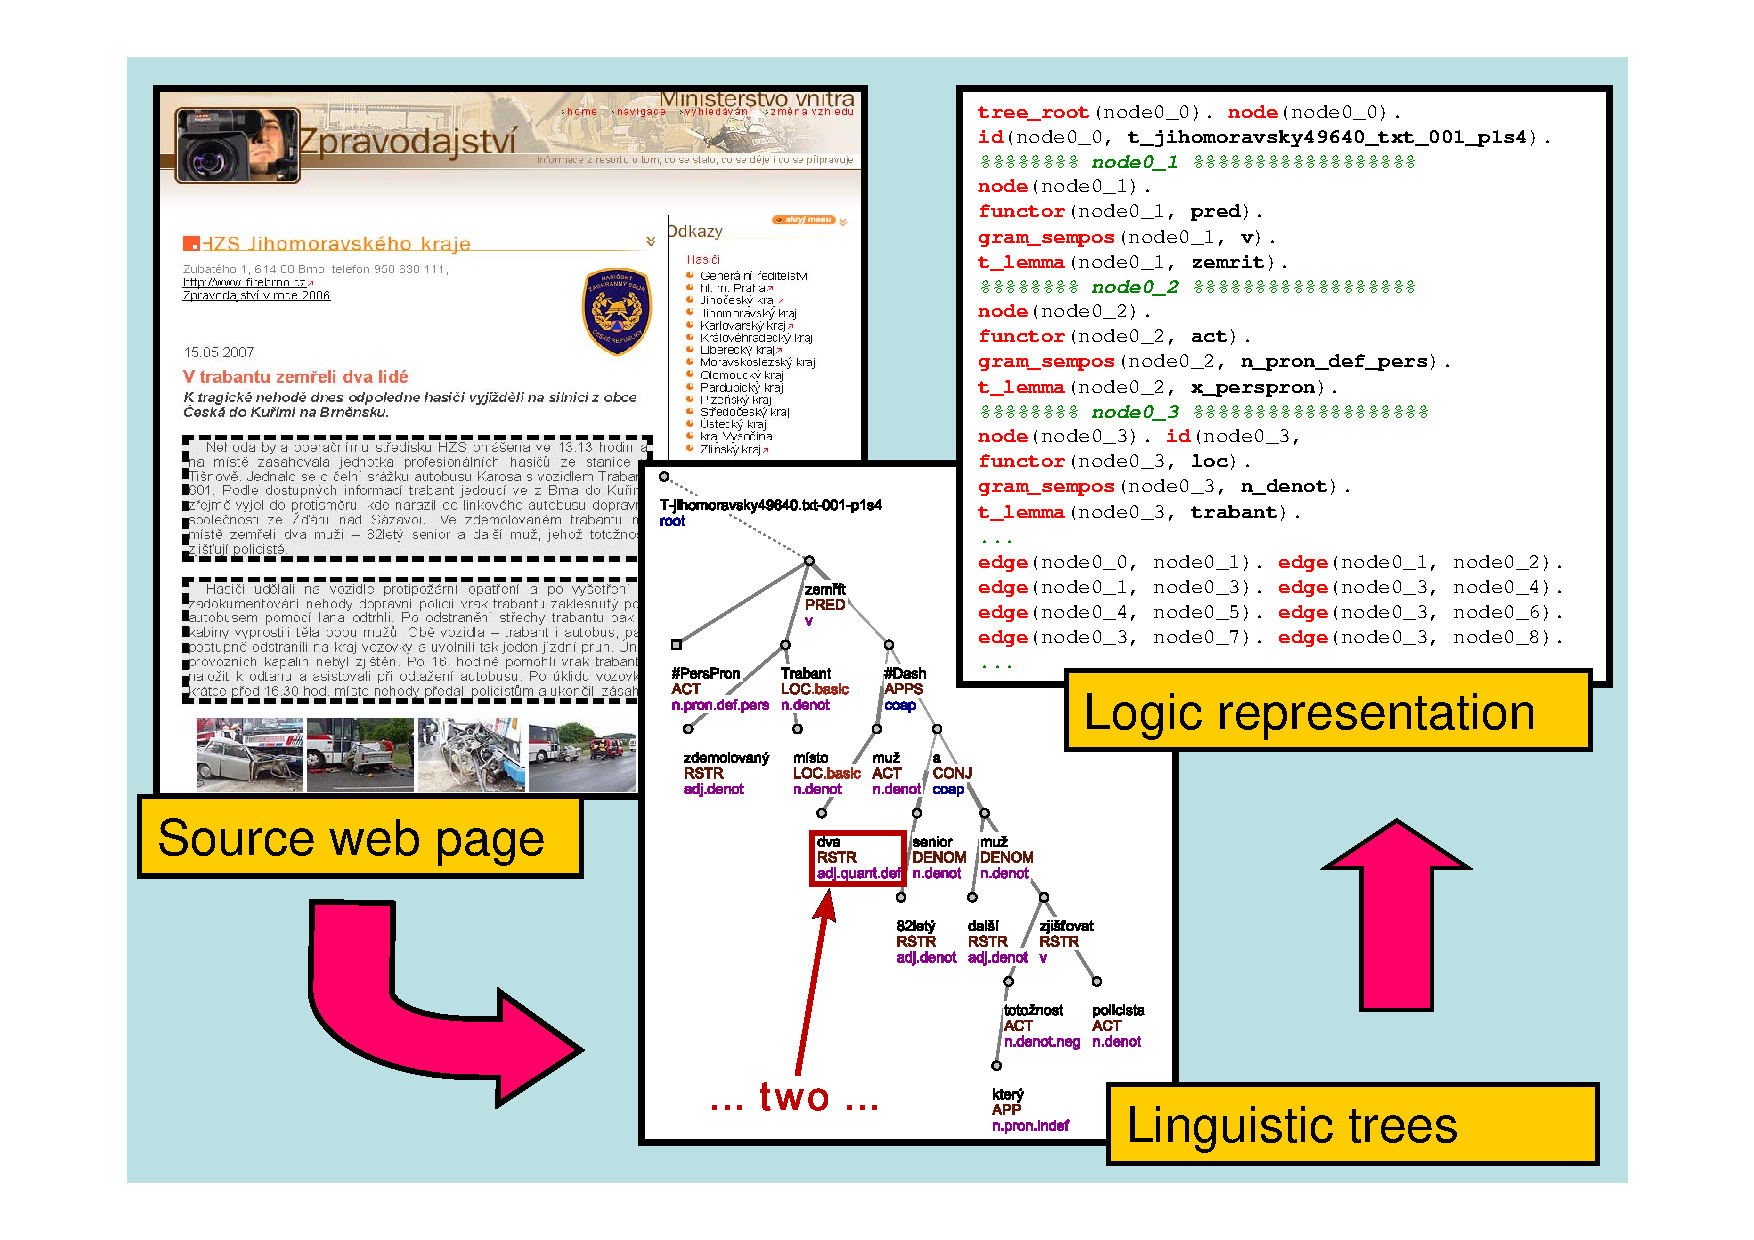
\includegraphics[height=0.9\hsize, angle=-90]{img/LogicRepresentation}}
\end{columns}
\end{frame}

\begin{frame}{Root/Subtree Preprocessing/Postprocessing}
\centerline{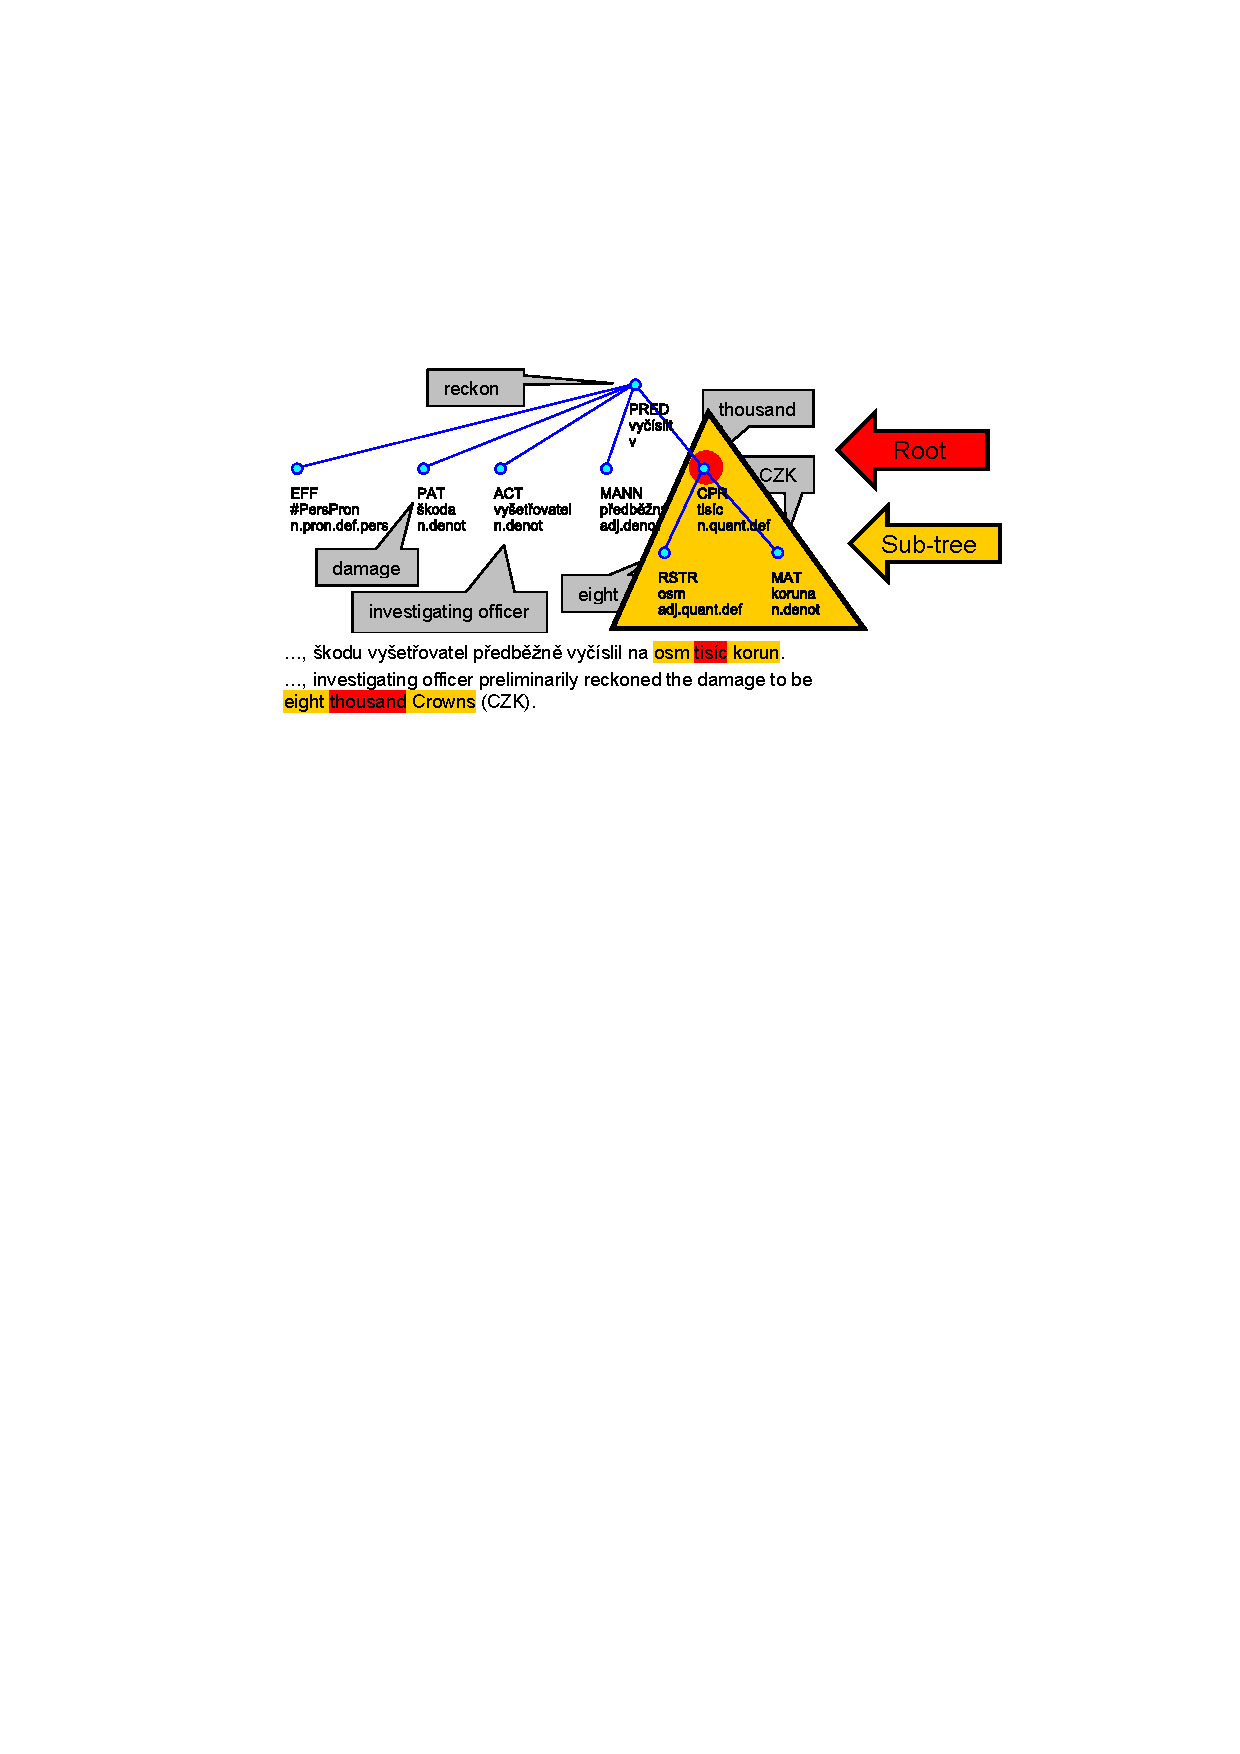
\includegraphics[width=\hsize]{img/tree-subtree}}
\bigskip
\begin{itemize}
	\item Multi-word expressions
\end{itemize}
\end{frame}


\begin{frame}[fragile]{Rules with largest coverage (Czech fireman dataset)}
\begin{minted}[linenos,  fontsize=\tiny, tabsize=3]{prolog}
% [cars - Rule 3] [Pos cover = 5 Neg cover = 0]
mention(cars,A) :-
   'lex.rf'(B,A), sempos(B,'n.denot'), tDependency(C,B), t_lemma(C,vozidlo), 
   functor(C,'ACT'), number(C,sg).   % vozidlo ~ vehicle
% [damage - Rule 1] [Pos cover = 14 Neg cover = 0]
mention(damage,A) :-
   'lex.rf'(B,A), sempos(B,'n.quant.def'), tDependency(C,B), tDependency(C,D), 
   t_lemma(D,'vyšetřovatel').   % vyšetřovatel ~ investigating officer
% [end_subtree - Rule 7] [Pos cover = 6 Neg cover = 0]
mention(end_subtree,A) :-
   'lex.rf'(B,A), sempos(B,'n.quant.def'), tDependency(C,B), t_lemma(C,'ukončit').
       % ukončit ~ finish
% [start - Rule 2] [Pos cover = 15 Neg cover = 0]
mention(start,A) :-
   'lex.rf'(B,A), functor(B,'TWHEN'), tDependency(C,B), tDependency(C,D), 
   t_lemma(D,ohlásit).   % ohlásit ~ report (e.g. a fire)
% [injuries - Rule 1] [Pos cover = 7 Neg cover = 0]
mention(injuries,A) :-
   'lex.rf'(B,A), functor(B,'PAT'), tDependency(B,C), t_lemma(C,'zraněný'), 
   tDependency(D,B), aspect(D,cpl).   % zraněný ~ injured
% [fatalities - Rule 1] [Pos cover = 3 Neg cover = 0]
mention(fatalities,A) :-
   'lex.rf'(B,A), functor(B,'PAT'), tDependency(C,B), t_lemma(C,srazit).
       % srazit ~ knock down
% [professional_unit - Rule 1] [Pos cover = 17 Neg cover = 0]
mention(professional_unit,A) :-
   'lex.rf'(B,A), functor(B,'LOC'), gender(B,fem), tDependency(C,B), 
   functor(C,'CONJ'), overlap_Lookup_tToken(D,B).
% [amateur_unit - Rule 1] [Pos cover = 19 Neg cover = 0]
mention(amateur_unit,A) :-
   'lex.rf'(B,A), tDependency(C,B), tDependency(D,C), tDependency(D,E), 
   t_lemma(E,dobrovolný).   % dobrovolný ~ voluntary
\end{minted}
\end{frame}

\begin{frame}{Evaluation -- Czech fireman -- Precision (optimistic example)}
\begin{tabular}
{lcrclcrcl@{\hspace{0.1cm}}cc}

\multicolumn{11}{c}{Strict Precision}\\
\hline
Task && \multicolumn{3}{c}{ILP}  && \multicolumn{3}{c}{PAUM} && \\
\hline
              cars &&      0.324 &  $\pm$  &       0.387 & &      0.380 &  $\pm$  &       0.249 &  \\
            damage &&      0.901 &  $\pm$  &       0.178 & &      0.860 &  $\pm$  &       0.176 &  \\
       end subtree &&      0.529 &  $\pm$  &       0.381 & &      0.499 &  $\pm$  &       0.242 &  \\
             start &&      0.929 &  $\pm$  &       0.109 & &      0.651 &  $\pm$  &       0.152 & $\bullet$ \\
          injuries &&      0.667 &  $\pm$  &       0.291 & &      0.398 &  $\pm$  &       0.205 & $\bullet$ \\
        fatalities &&      0.814 &  $\pm$  &       0.379 & &      0.307 &  $\pm$  &       0.390 & $\bullet$ \\
  rofessional unit &&      0.500 &  $\pm$  &       0.241 & &      0.677 &  $\pm$  &       0.138 & $\circ$ \\
      amateur unit &&      0.863 &  $\pm$  &       0.256 & &      0.546 &  $\pm$  &       0.293 & $\bullet$ \\
\hline
           overall &&      0.691 &  $\pm$  &       0.358 & &      0.540 &  $\pm$  &       0.297 & $\bullet$ \\
\hline
\multicolumn{11}{c}{$\circ$, $\bullet$ statistically significant improvement or degradation}\\
\end{tabular}
\end{frame}

\begin{frame}{Evaluation -- Corporate acquisitions -- Overall}
\small
\begin{tabular}{|l|r>{\columncolor{lightgray}}r|ccc>{\columncolor{lightgray}}ccc|}
\hline%
& \multicolumn{2}{c|}{Annotations} & \multicolumn{6}{c|}{Extraction Method}\\
Task 				 &  ver. A 				 &  ver. B 				 &  SRV  					 &  HMM 				  &  Elie				  &  SVM+ILP			  &  ILP				  &  PAUM\\\hline%\\
acquired		 &  \textbf{683} 	 &  651 					 &  38.5 					 &  \emph{30.9}	  &  43.5				  &  41.8					  &  31.3				  & \textbf{47.3}\\
acqabr   		 &  \textbf{1450}  &  1494					 &  38.1 					 &  40.1 				  &  39.7				  &  42.6					  &  \emph{25.8}  & \textbf{45.6}\\
purchaser 	 &  \textbf{624} 	 &  594 					 &  45.1 					 &  48.1				  &  46.2				  &  45.4					  &  \emph{36.7}  & \textbf{51.1}\\
purchabr 		 &  1263 					 &  \textbf{1347}  &  \textbf{48.5}	 &  n/a 				  &  28.7				  &  35.4					  &  \emph{17.2}  & 44.3\\
seller 			 &  267 					 &  \textbf{707} 	 &  23.4 					 &  n/a 				  &  \emph{15.6}  &  \textbf{51.5}  &  17.0				  & 23.2\\
sellerabr 	 &  431 					 &  \textbf{458} 	 &  \textbf{25.1}  &  n/a 				  &  13.4 			  &  21.7 				  &  \emph{8.5}	  & 20.2\\
dlramt 			 &  \textbf{283} 	 &  206 					 &  61.8 					 &  55.3 				  &  59.0				  &  53.0 				  &  \emph{28.0}  & \textbf{65.9}\\\hline%\\
Total/Overall&  5001 					 &  \textbf{5457}	 &  41.1 					 &  n/a				 	  &  33.5				  &  40.8					  &  \emph{23.9}  & \textbf{44.0}\\
\hline%
\end{tabular}	

\begin{itemize}
	\item $F_1$ measure
	\item Two versions of the dataset (A - white / B - gray) 
	\item Results taken form the literature (except ILP and PAUM)
	\bigskip
	\item ``Baseline experiments'', see also the discussion slide (\pageref{future_experiments}) about future experimenting possibilities
\end{itemize}

\end{frame}


\subsection{Shareable Extraction Ontologies}
\themecolor{\colorShareable}
\frame{\frametitle{Shareable Extraction Ontologies} \tableofcontents[currentsection, currentsubsection]}

\begin{frame}{Extraction Ontology}  
\begin{itemize}
	\item The knowledge (extraction model) used in the extraction process can itself be saved in an ontology.
	\begin{itemize}
		\item So called Extraction Ontology
	\end{itemize}
	\bigskip
	\item D.~W. Embley, ``Toward semantic understanding: an approach based on \alert{information
  extraction ontologies},'' in \emph{ADC '04}.\hskip 1em plus 0.5em minus
  0.4em\relax Darlinghurst: ACS, 2004, pp. 3--12.
	\item M.~{Labsk\'{y} et al.}, ``{The Ex Project: Web Information Extraction Using
  \alert{Extraction Ontologies}},'' in \emph{Knowledge Discovery Enhanced with Semantic
  and Social Information}, ser. Studies in Comput. Intellig.\hskip 1em plus
  0.5em minus 0.4em\relax Springer, 2009, vol. 220, pp. 71--88.
	\bigskip
	\item But these Extraction Ontologies can only be used with the original tool.
	\item They are not shareable!
\end{itemize}
\end{frame}


\begin{frame}{Extraction Rules Interpreted by OWL Reasoner}
\centerline{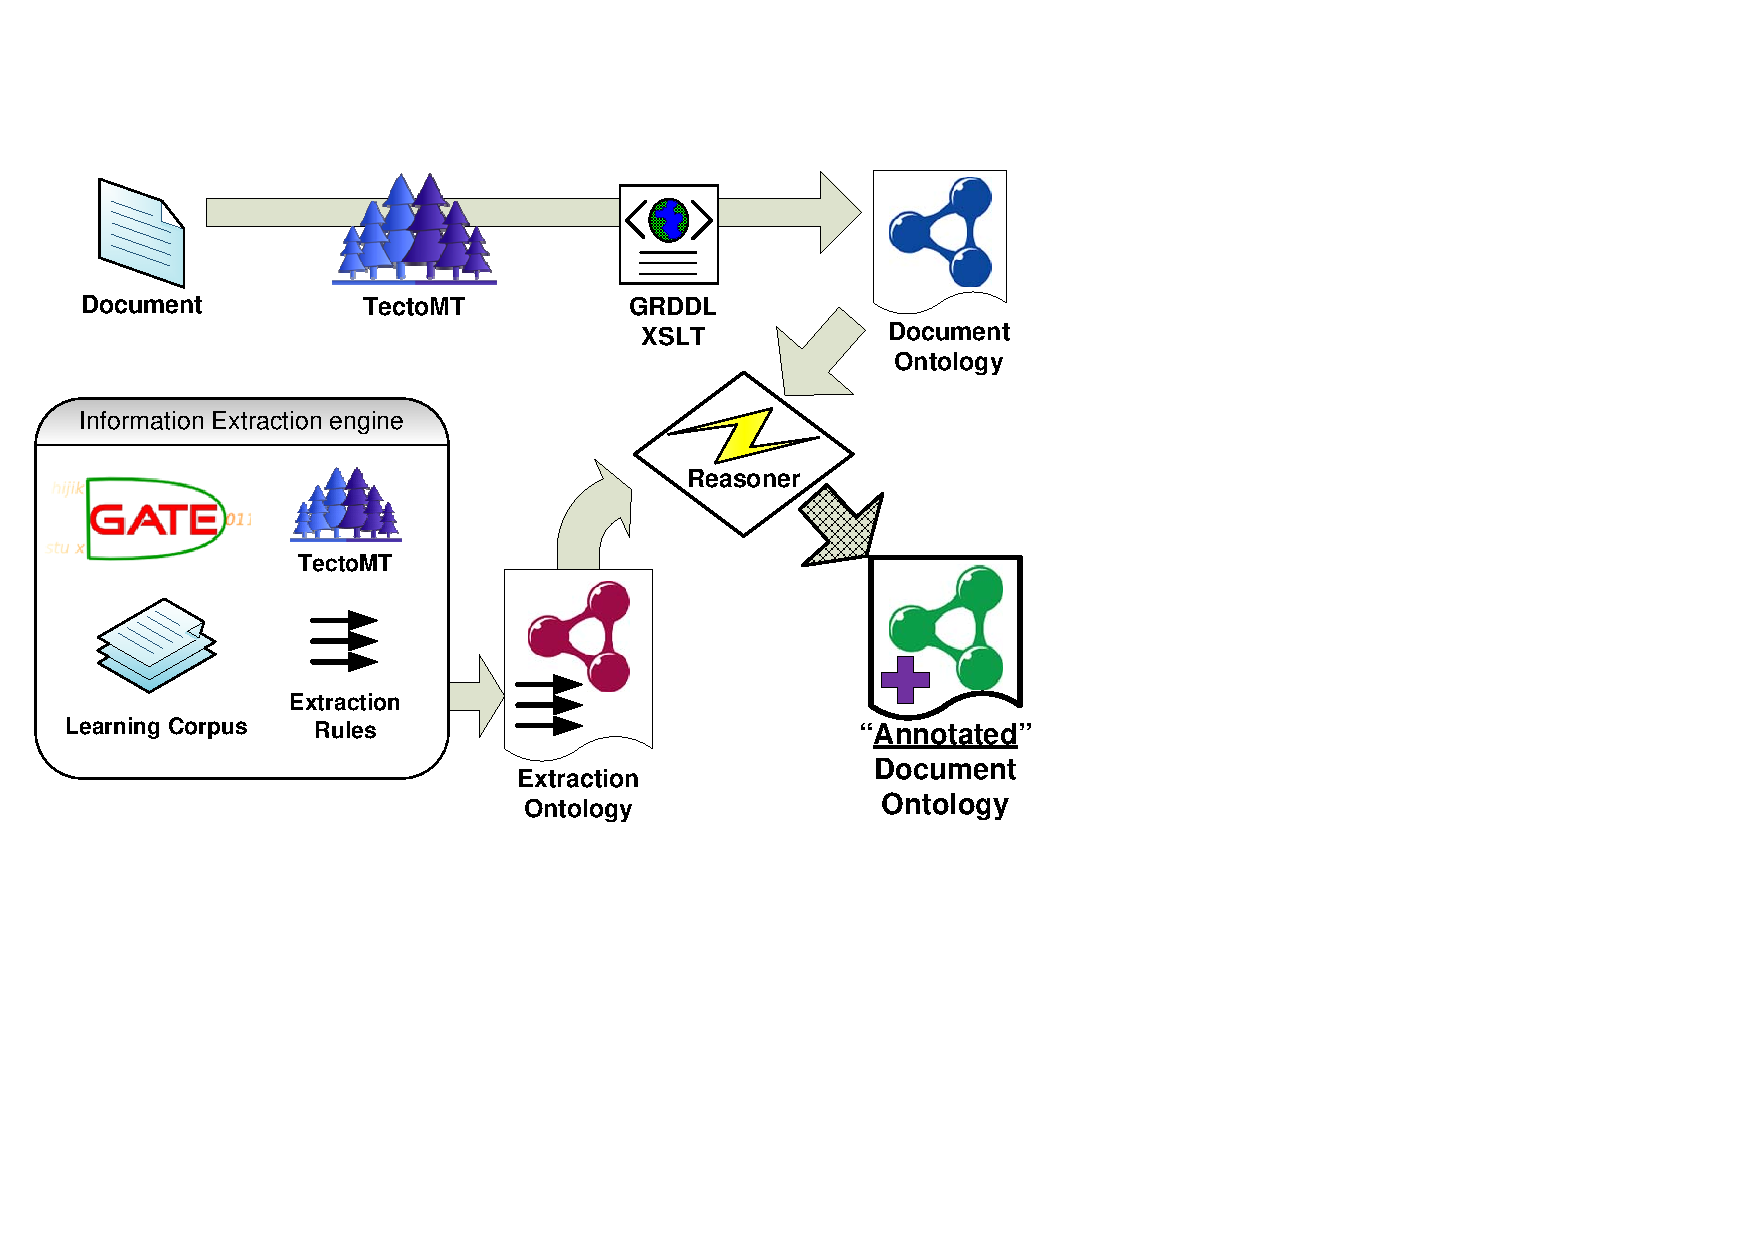
\includegraphics[width=0.7\vsize, angle=-90]{img/semantic_rules_app_schema}}
\medskip
\begin{itemize}
	\item Tool \alert{independent} extraction ontologies
\end{itemize}
\end{frame}

\begin{frame}[fragile]{Extraction rules in OWL/XML syntax for Rules}
\begin{minted}[linenos,  fontsize=\tiny, tabsize=3]{xml}
<?xml version="1.0" encoding="UTF-8"?>
<!DOCTYPE Ontology [
   <!ENTITY pml "http://ufal.mff.cuni.cz/pdt/pml/" >
]>
<Ontology xmlns="http://www.w3.org/2002/07/owl#"
   ontologyIRI="http://czsem.berlios.de/ontologies/...rules.owl">
   <DLSafeRule>
      <Body>
         <ObjectPropertyAtom> <ObjectProperty IRI="&pml;lex.rf"/>
            <Variable IRI="urn:swrl#b"/> <Variable IRI="urn:swrl#a"/>
         </ObjectPropertyAtom>
         <DataPropertyAtom> <DataProperty IRI="&pml;sempos"/>
            <Variable IRI="urn:swrl#b"/> <Literal>n.quant.def</Literal>
         </DataPropertyAtom>
         <ObjectPropertyAtom> <ObjectProperty IRI="&pml;tDependency"/>
            <Variable IRI="urn:swrl#c"/> <Variable IRI="urn:swrl#b"/>
         </ObjectPropertyAtom>
         <ObjectPropertyAtom> <ObjectProperty IRI="&pml;tDependency"/>
            <Variable IRI="urn:swrl#c"/> <Variable IRI="urn:swrl#d"/>
         </ObjectPropertyAtom>
         <DataPropertyAtom> <DataProperty IRI="&pml;t_lemma"/>
            <Variable IRI="urn:swrl#d"/> <Literal>vyšetřovatel</Literal>
         </DataPropertyAtom>
      </Body>
      <Head>
         <DataPropertyAtom> <DataProperty IRI="&pml;mention_root" />
            <Literal>damage</Literal> <Variable IRI="urn:swrl#a" />
         </DataPropertyAtom>
      </Head>
   </DLSafeRule>
</Ontology>
\end{minted}
\end{frame}

\begin{frame}[fragile]{Extraction rules in Prot\'{e}g\'{e}}
\begin{minted}[linenos,  fontsize=\small, tabsize=3]{jena}
#[Rule 1]
lex.rf(?b, ?a), sempos(?b, "n.quant.def"), tDependency(?c, ?b),
tDependency(?c, ?d), t_lemma(?d, "vyšetřovatel") #investigator
      -> mention_root(?a, "damage")

#[Rule 2]
lex.rf(?b, ?a), functor(?b, "TOWH"), tDependency(?c, ?b),
tDependency(?c, ?d), t_lemma(?d, "škoda") #damage
      -> mention_root(?a, "damage")
\end{minted}
\end{frame}

\begin{frame}[fragile]{Extraction rules in Jena}
\begin{minted}[linenos,  fontsize=\small, tabsize=3]{jena}
@prefix pml: <http://ufal.mff.cuni.cz/pdt/pml/>.
[rule-1:  
        ( ?b pml:lex.rf ?a )
        ( ?b pml:sempos 'n.quant.def' )
        ( ?c pml:tDependency ?b )
        ( ?c pml:tDependency ?d )
        ( ?d pml:t_lemma 'vyšetřovatel' )
     -> 
        ( ?a pml:mention_root 'damage' )
]
\end{minted}
\end{frame}



\begin{frame}{Performance Evaluation -- Datasets \& Reasoners}
\centerline{
\begin{tabular}{|r||l|l|b{7mm}|b{7mm}|b{7mm}|}
\hline
\alert{dataset} & domain & language & num of files &  data size (MB) &  num of rules  \\
\hline
\hline
\textbf{czech\_fireman} & accidents & Czech &  50 &  16 &  2\\
\hline
\textbf{acquisitions} & finance & English &  600 &  126 &  113\\
\hline
\end{tabular}
}
\bigskip
\centerline{
\begin{tabular}{|r||r|r||r|r|}
\hline
\alert{reasoner} & \textbf{czech\_fireman} & stdev & \textbf{acquisitions-v1.1} & stdev\\
\hline
\hline
\textbf{Jena} & 161 s & 0.226 & 1259 s & 3.579\\
\hline
\textbf{HermiT} & 219 s & 1.636 & $\gg$ 13 hours & \\
\hline
\textbf{Pellet} & 11 s & 0.062 & 503 s & 4.145\\
\hline
\textbf{FaCT++} & \multicolumn{4}{|c|}{Does not support rules.}\\
\hline
\end{tabular}
}
\bigskip
\begin{itemize}
	\item Poor performance\dots
	\item Because these tools are not optimized for these taks (yet?)
\end{itemize}
\end{frame}


\subsection{Fuzzy ILP Document Classification}
\themecolor{\colorFuzzy}
\frame{\frametitle{Fuzzy ILP Document Classification} \tableofcontents[currentsection, currentsubsection]}

\begin{frame}{Schema of the whole system}
\begin{columns}
\column{.45\textwidth}
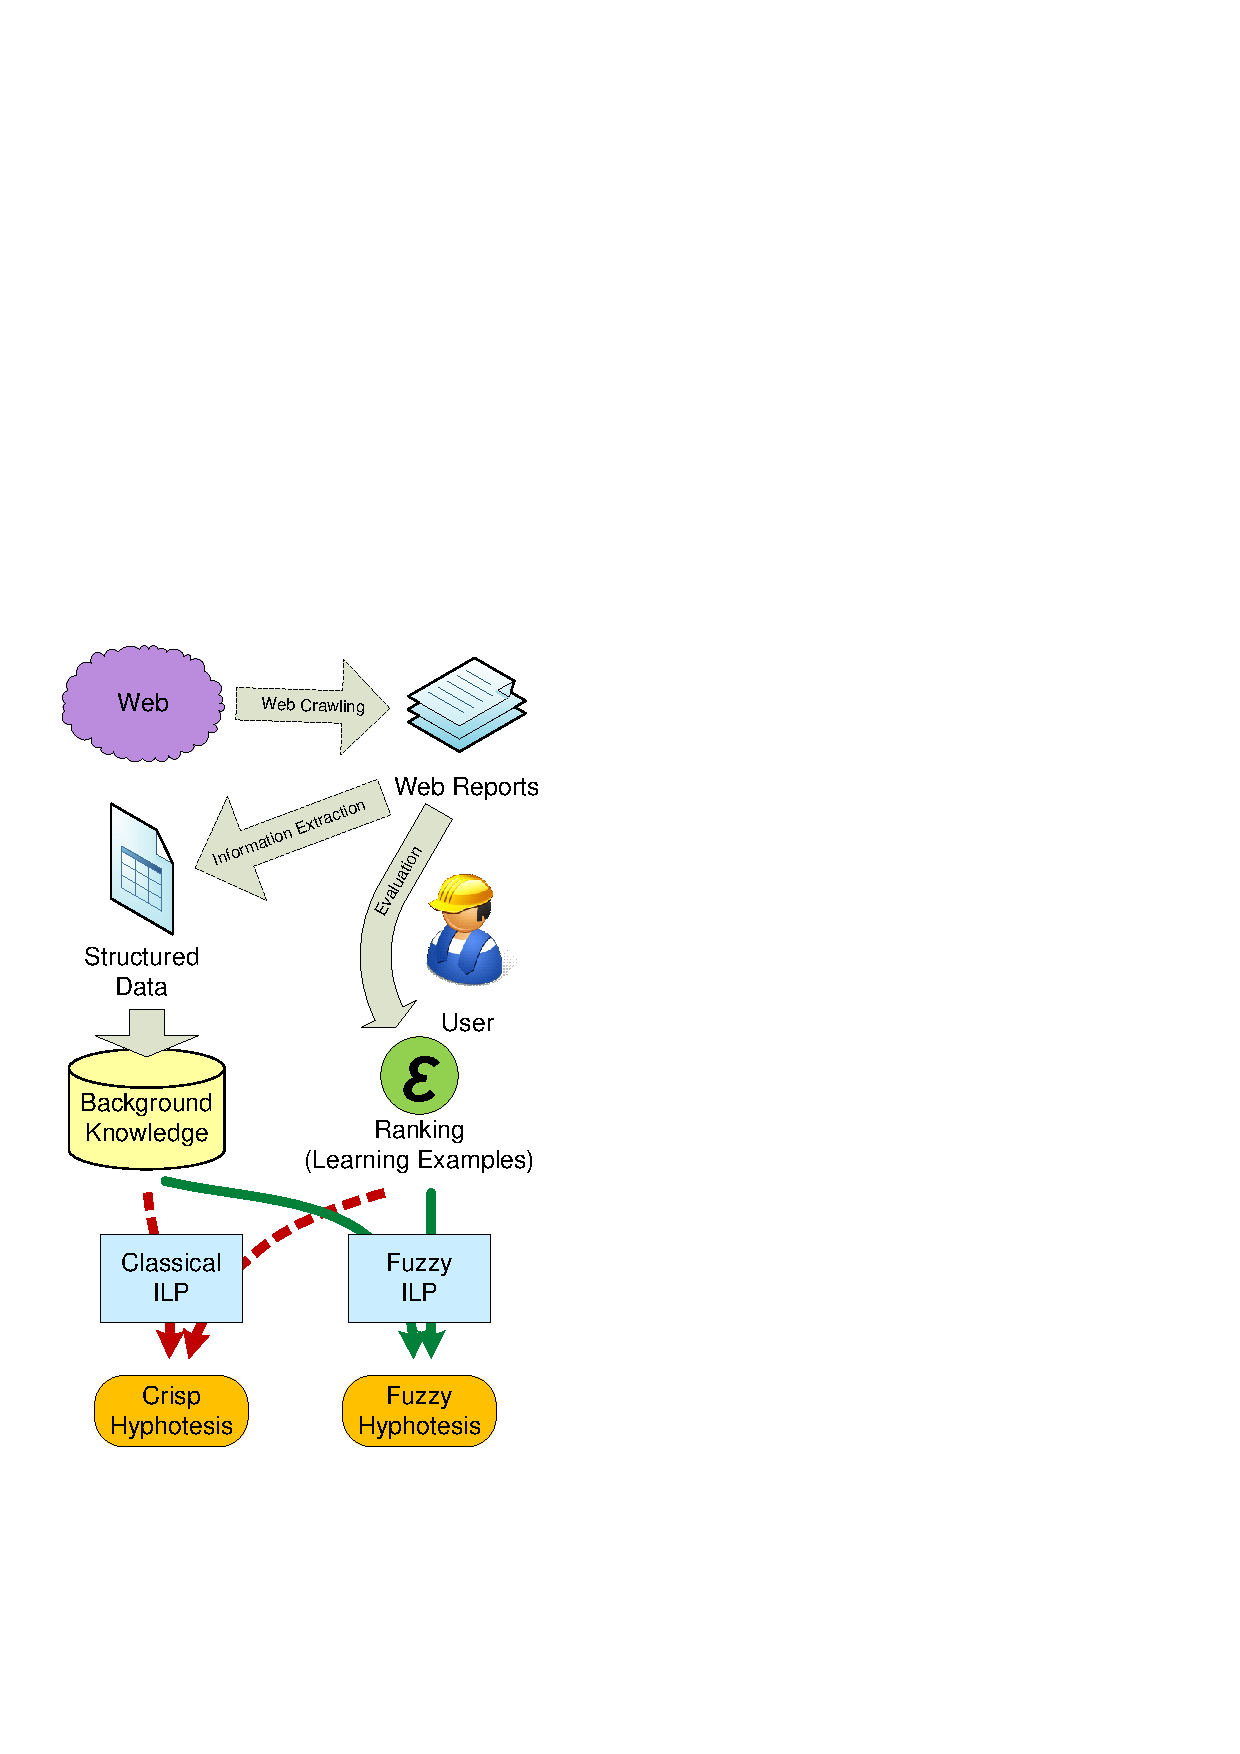
\includegraphics[height=0.9\vsize]{img/fuzzy_schema}
\column{.55\textwidth}
\begin{enumerate}
	\item Web Crawling
	\item Information Extraction and User Evaluation
	\item Logic representation
		\begin{itemize}
			\item Construction of \alert{background knowledge}
			\item Construction of \alert{learning examples}
		\end{itemize}
	\item ILP Learning
		\begin{itemize}
			\item Crisp
			\item Fuzzy
		\end{itemize}
		
	\bigskip
	\item Comparison of results
\end{enumerate}
\end{columns}
\end{frame}

\begin{frame}[fragile]{Essential difference between learning examples}
\begin{columns}
\column{.6\textwidth}
\setbeamercolor{block title}{bg=BrickRed}
\begin{block}{Crisp learning examples}
\begin{minted}[fontsize=\footnotesize]{prolog}
serious_2(id_47443). %positive
 
serious_0(id_47443). %negative
serious_1(id_47443). %negative
serious_3(id_47443). %negative
\end{minted}
\end{block}
\bigskip
\setbeamercolor{block title}{bg=OliveGreen}
\begin{block}{Monotonized learning examples}
\begin{minted}[fontsize=\footnotesize]{prolog}
serious_atl_0(id_47443). %positive
serious_atl_1(id_47443). %positive
serious_atl_2(id_47443). %positive
 
serious_atl_3(id_47443). %negative
\end{minted}
\end{block}
\column{.4\textwidth}
\begin{itemize}
	\item For one evidence (occurrence, e.g. one accident)
	\bigskip
	\item Crisp:\\
	Always \alert{one} positive and \alert{three} negative learning examples
	\bigskip
	\item Monotonized:\\
	\alert{Up to the observed degree} positive,\\the rest negative.
\end{itemize}
\end{columns}
\end{frame}

\begin{frame}[fragile]{Monotonization of attributes}
\definecolor{MyBrown}{rgb}{0.5,0.5,0}
\setbeamercolor{block title}{bg=MyBrown}
\begin{block}{damage\_atl $\leftarrow$ damage}
\begin{minted}[fontsize=\footnotesize]{prolog}
damage_atl(ID,N) :- damage(ID,N), not(integer(N)). %unknown values

damage_atl(ID,N) :- damage(ID,N2), integer(N2), %numeric values
                    damage(N), integer(N), N2>=N.
\end{minted}
\end{block}
\bigskip
\begin{itemize}
	\item We infer all lower values as sufficient.
	\item Treatment of unknown values.
	\item Negation as failure.
\end{itemize}
\end{frame}

\begin{frame}[fragile]{Rules for the whole Czech fireman dataset}
\begin{minted}[linenos,  fontsize=\tiny, tabsize=3]{prolog}
% Crisp
serious_0(A) :- fatalities(A,0), injuries(A,0), cars(A,1), 
                amateur_units(A,0), lather(A,0).
serious_0(A) :- fatalities(A,0), cars(A,0), amateur_units(A,0),
                professional_units(A,1).
serious_1(A) :- amateur_units(A,1).
serious_1(A) :- damage(A,300000).
serious_1(A) :- type(A,fire), amateur_units(A,0), pipes(A,2).
serious_1(A) :- type(A,car_accident), dur_minutes(A,unknown),
                fatalities(A,0), injuries(A,1).
serious_2(A) :- lather(A,unknown).
serious_2(A) :- cars(A,0), lather(A,0), aqualung(A,1), fan(A,0).
serious_2(A) :- amateur_units(A,2).
serious_3(A) :- fatalities(A,2).
serious_3(A) :- type(A,fire), dur_minutes(A,unknown), cars(A,0), fan(A,0).
serious_3(A) :- injuries(A,2), cars(A,2).
serious_3(A) :- fatalities(A,1).

% Monotonized
serious_atl_0(A).
serious_atl_1(A) :- injuries_atl(A,1).
serious_atl_1(A) :- dur_minutes_atl(A,21), pipes_atl(A,1), aqualung_atl(A,0).
serious_atl_1(A) :- damage_atl(A,8000), amateur_units_atl(A,3).
serious_atl_1(A) :- dur_minutes_atl(A,197).
serious_atl_1(A) :- dur_minutes_atl(A,unknown).
serious_atl_2(A) :- dur_minutes_atl(A,50), pipes_atl(A,3).
serious_atl_2(A) :- size_atl(A,1364), injuries_atl(A,1).
serious_atl_2(A) :- fatalities_atl(A,1).
serious_atl_2(A) :- size_atl(A,1106), professional_units_atl(A,3).
serious_atl_3(A) :- fatalities_atl(A,1).
serious_atl_3(A) :- damage_atl(A,1500000).
\end{minted}
\end{frame}



\begin{frame}[fragile]{Conversion of Results}
\setbeamercolor{block title}{bg=OliveGreen}
\begin{block}{serious\_t $\leftarrow$ serious\_atl\_t \phantom{X} (selecting maximum)}
\begin{minted}[fontsize=\footnotesize]{prolog}
serious_0(ID) :- serious_atl_0(ID),
                 not(serious_atl_1(ID)), not(serious_atl_2(ID)),
                 not(serious_atl_3(ID)).
serious_1(ID) :- serious_atl_1(ID),
                 not(serious_atl_2(ID)), not(serious_atl_3(ID)).
serious_2(ID) :- serious_atl_2(ID),
                 not(serious_atl_3(ID)).
serious_3(ID) :- serious_atl_3(ID).
\end{minted}
\end{block}
\end{frame}




\begin{frame}{Evaluation -- Czech fireman dataset}
%\hspace*{-0.8cm}
\scriptsize
{\centering \begin{tabular}{lr@{\hspace{0cm}}c@{\hspace{0cm}}rr@{\hspace{0cm}}c@{\hspace{0cm}}r@{\hspace{0.05cm}}cr@{\hspace{0cm}}c@{\hspace{0cm}}r@{\hspace{0.05cm}}cr@{\hspace{0cm}}c@{\hspace{0cm}}r@{\hspace{0.05cm}}cr@{\hspace{0cm}}c@{\hspace{0cm}}r@{\hspace{0.05cm}}cr@{\hspace{0cm}}c@{\hspace{0cm}}r@{\hspace{0.05cm}}cr@{\hspace{0cm}}c@{\hspace{0cm}}r@{\hspace{0.05cm}}c}
\\
\hline
& \multicolumn{3}{c}{Fuzzy}& \multicolumn{4}{c}{Crisp} & \multicolumn{4}{c}{MultPerc} & \multicolumn{4}{c}{SMO} & \multicolumn{4}{c}{J48} & \multicolumn{4}{c}{JRip} & \multicolumn{4}{c}{LBoost} \\
\hline
Corr	& 0.61 & $\pm$ & .19 & .22 & $\pm$ & .17 & $\bullet$ & .41 & $\pm$ & .19 & $\bullet$ & .36 & $\pm$ & .24 & $\bullet$ & .41 & $\pm$ & .22 & $\bullet$ & .44 & $\pm$ & .17 & $\bullet$ & .59 & $\pm$ & .26 &        \\
Incor	& .39 & $\pm$ & .19 & .27 & $\pm$ & .24 &         	& .59 & $\pm$ & .19 & $\circ$ 	& .64 & $\pm$ & .24 & $\circ$ 	& .59 & $\pm$ & .22 & $\circ$ 	& .56 & $\pm$ & .17 & $\circ$ 	& .41 & $\pm$ & .26 &        \\
Uncl	& .00	& $\pm$ & .00	& .51 & $\pm$ & .29 & $\circ$ 	& .00 & $\pm$ & .00 &         	& .00 & $\pm$ & .00 &         	& .00 & $\pm$ & .00 &         	& .00 & $\pm$ & .00 &         	& .00 & $\pm$ & .00 &        \\
Prec	& .56 & $\pm$ & .24 & .53 & $\pm$ & .37 &         	& .35 & $\pm$ & .20 & $\bullet$ & .33 & $\pm$ & .26 &         	& .39 & $\pm$ & .22 &         	& .34 & $\pm$ & .21 & $\bullet$ & .56 & $\pm$ & .28 &        \\
Rec		& .61 & $\pm$ & .19 & .49 & $\pm$ & .32 &         	& .41 & $\pm$ & .19 & $\bullet$ & .36 & $\pm$ & .24 & $\bullet$ & .41 & $\pm$ & .22 & $\bullet$ & .44 & $\pm$ & .17 & $\bullet$ & .59 & $\pm$ & .26 &        \\
F			& .56 & $\pm$ & .20 & .49 & $\pm$ & .33 &         	& .36 & $\pm$ & .19 & $\bullet$ & .32 & $\pm$ & .24 & $\bullet$ & .39 & $\pm$ & .21 &         	& .36 & $\pm$ & .19 & $\bullet$ & .56 & $\pm$ & .27 &        \\
\hline
\multicolumn{21}{c}{$\circ$, $\bullet$ statistically significant improvement or degradation}\\
\end{tabular} \scriptsize \par}
\scriptsize
\smallskip
{\centering
\begin{tabular}{p{2cm}@{}p{10.5cm}}\\
Fuzzy \dotfill{}& czsem.ILP.FuzzyILPClassifier\\
Crisp \dotfill{} & czsem.ILP.CrispILPClassifier\\
MultPerc \dotfill{} & functions.MultilayerPerceptron\\
SMO \dotfill{} & functions.SMO\\
J48 \dotfill{} & trees.J48\\
JRip \dotfill{} & rules.JRip\\
LBoost \dotfill{} & meta.LogitBoost\\
\\
Corr \dotfill{} & Percent correct\\
Inor \dotfill{} & Percent incorrect\\
Uncl \dotfill{} & Percent unclassified\\
Prec \dotfill{} & Weighted avg IR precision\\
Rec \dotfill{} 	& Weighted avg IR recall\\
F \dotfill{} 		& Weighted avg F measure\\
\end{tabular}
}
%\caption{Evaluation of the methods in 2 times 10-fold cross validation.}
\end{frame}

\begin{frame}{Evaluation -- Czech fireman dataset}
\centerline{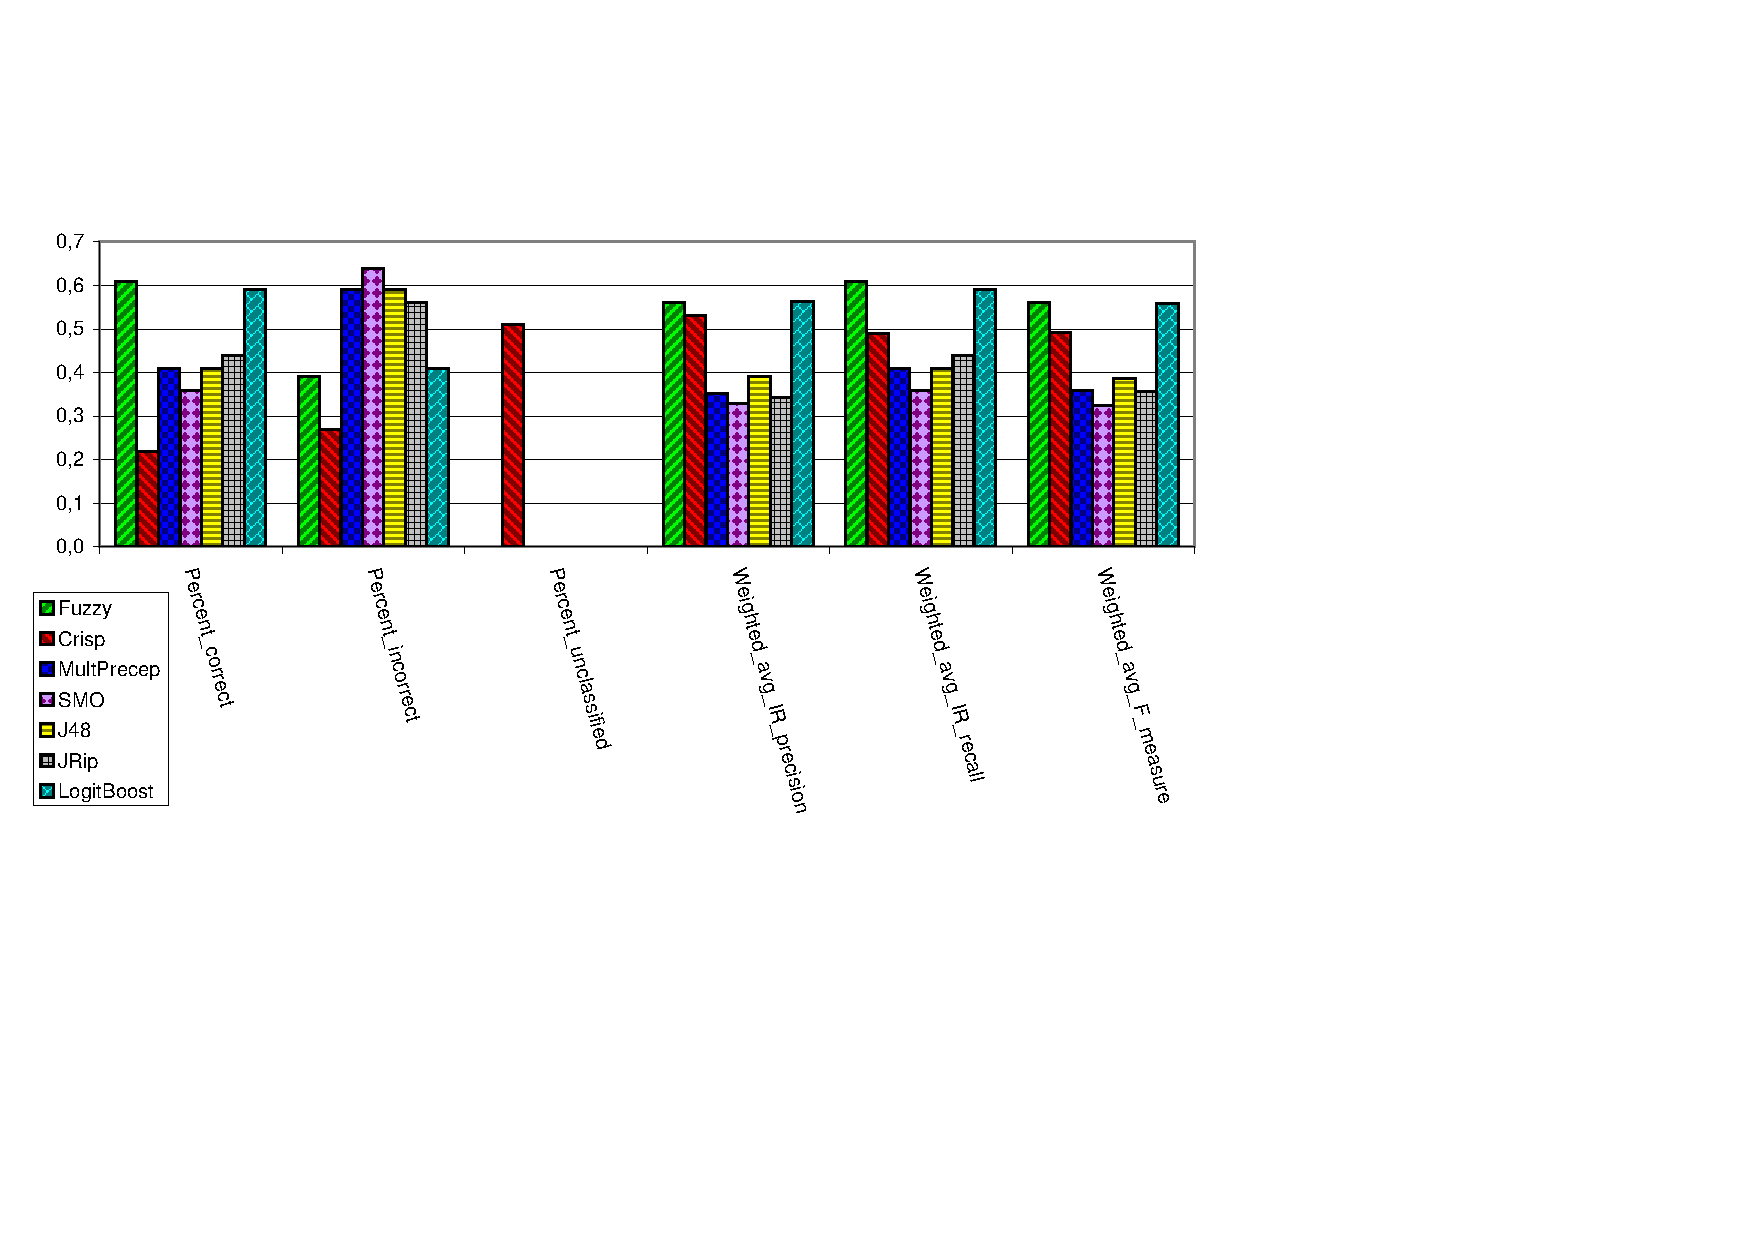
\includegraphics[height=1.0\hsize, angle=-90]{img/fuzzy_2x10cross}}
\end{frame}

\begin{frame}{The impact of dataset size on classification performance}
\centerline{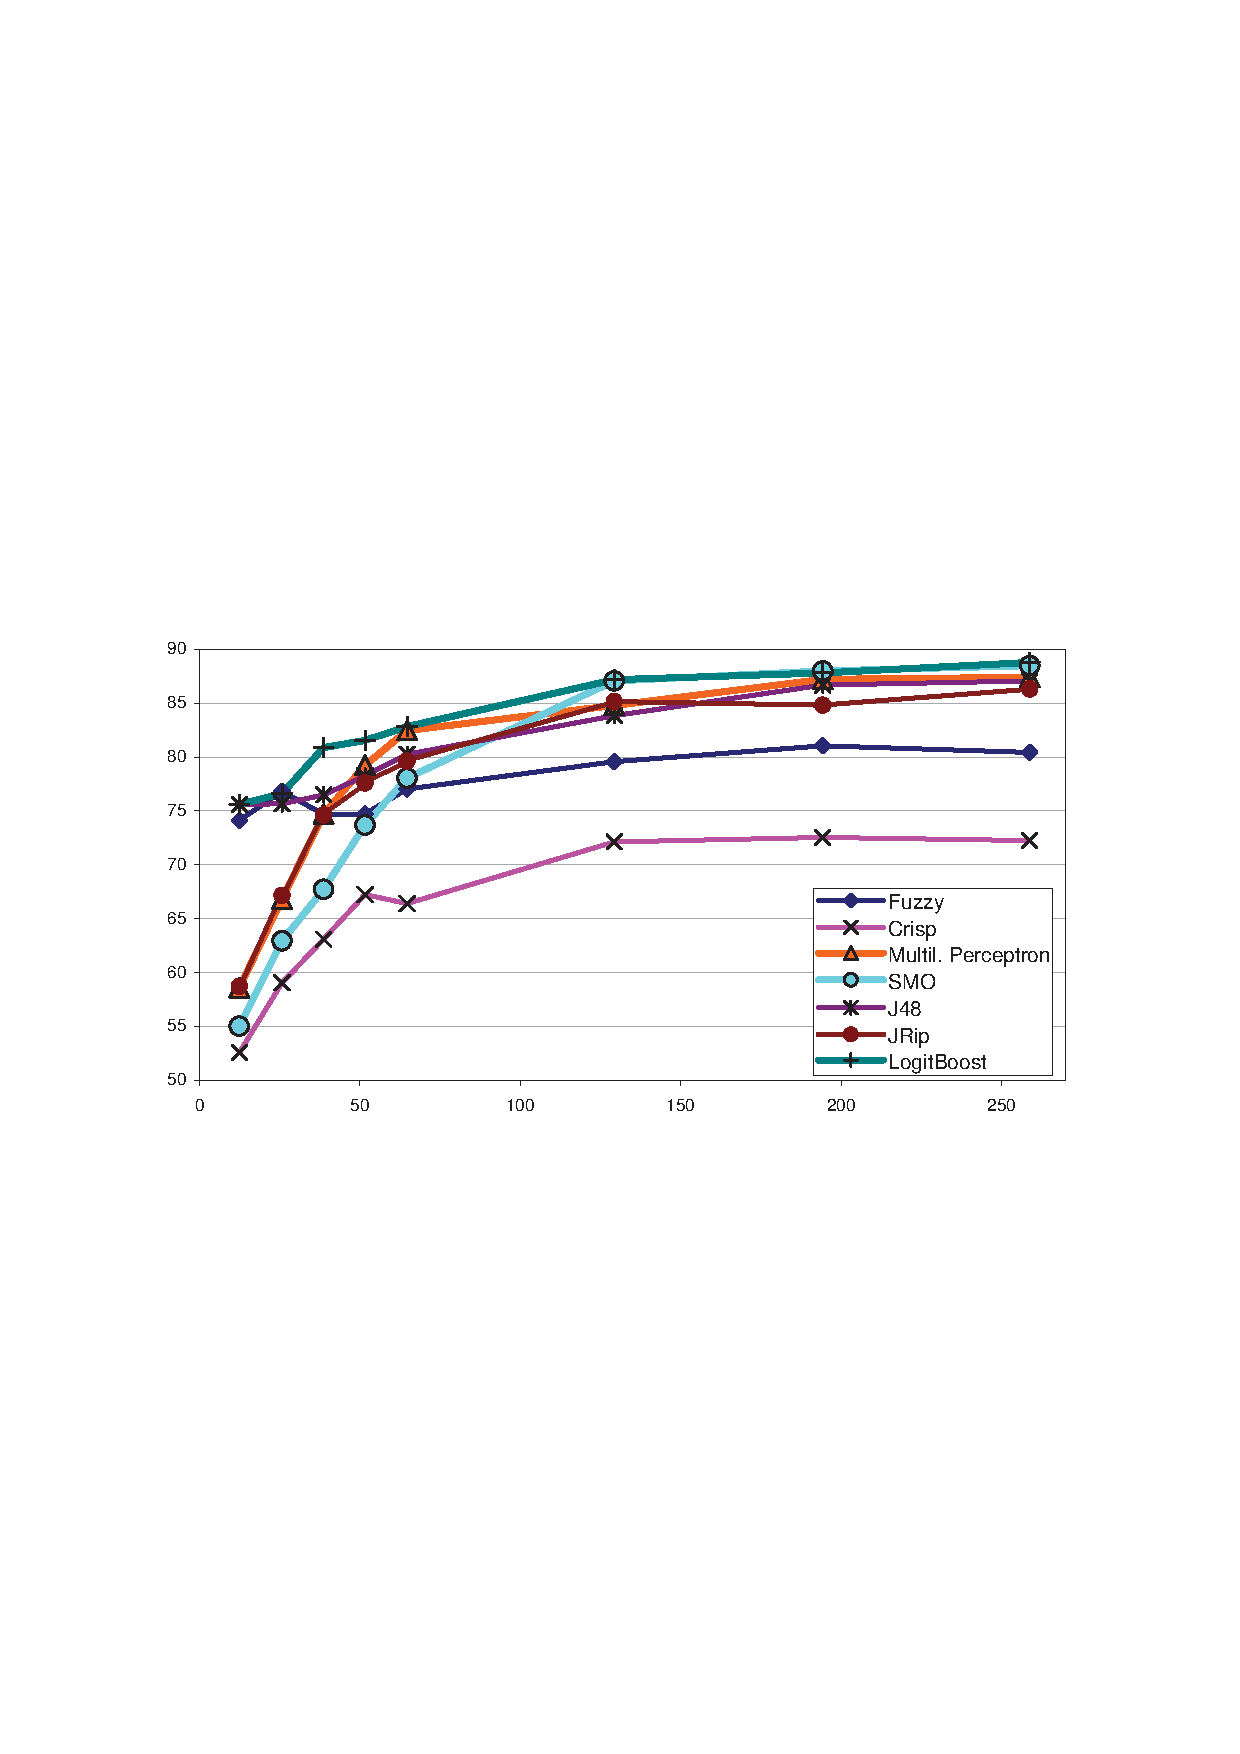
\includegraphics[width=1.0\hsize]{img/corect_growing_learninig_instances}}

\begin{itemize}
	\item `nursery' dataset from UCI ML Repository
	\item x-axis: number of training instances
	\item y-axis: percent of correctly classified instances
	\item average values from 10 repetitions
\end{itemize}

\end{frame}





\resetcolor
\section[Questions \& Comments]{Questions and Comments from Reviews} 
\frame{\tableofcontents[currentsection]}


\begin{frame}{The Title}
\begin{itemize}
	\item Nobody is happy with the title!
	\begin{itemize}
		\item Including the author himself \dots
	\end{itemize}
	\bigskip
	\item But it is quite difficult to find better one.
	\bigskip
	\item ``Use of deep language parsing for generation of extraction rules''
	\begin{itemize}
		\item The last two topics are not cowered
	\end{itemize}
	\item ``How ILP and ontologies can help information extraction''
	\begin{itemize}
		\item The first and the last topic is not cowered
	\end{itemize}
\end{itemize}
\end{frame}



\subsection{Review 1 (Filip Železný)} 
\frame{\tableofcontents[currentsection, currentsubsection]}

\subsection{Review 2 (Diana Maynard)} 
\frame{\tableofcontents[currentsection, currentsubsection]}

\themecolor{\colorLearning}
\begin{frame}{Topics / Questions / State-of-the-art}
\begin{itemize}
	\item The thesis consists of \alert{four equally important topics}
	\item We cannot concentrate on a single one (\themetext[colorLearning]{Induction of Extraction Rules})
	\bigskip
	\item There are many questions in the review
	\begin{itemize}
		\item Let us go through them, \alert{they all can be resolved!}
	\end{itemize}
	\bigskip
	\item It was really had work to prepare and evaluate the baseline method
	\item And make it \alert{directly comparable} with the state-of-the-art solutions
	\item The framework is now open to everybody
	\item ``Infinite'' amount of experiments can be performed
	\begin{itemize}
		\item See also the discussion slide (\pageref{future_experiments}) about future experimenting possibilities and their \alert{complexity}
	\end{itemize}
\end{itemize}
\end{frame}
\resetcolor


\begin{frame}{The Task of Information Extraction}
\begin{quotation}
\small The task of IE should be clearly defined, making clear what it involves, why it is needed, and why it is hard. ... Sections on IE components ... are much too short. ... I would expect these issues to be covered and discussed in depth, with appropriate references (these issues have all been discussed many times in the literature), ...
\end{quotation}

\begin{itemize}
	\item Is it really necessary to discuss all these topics?	
	\begin{itemize}
		\item It concerns only 2 of 4 main topics of the thesis.
		\item We are not creating a text book, are we?
		\item What is the contribution in it?
	\end{itemize}	
	\item What reference is actually missing?
	\item Is the used terminology lacking something important?
\end{itemize}
\begin{center}
	\begin{tabular}{l|l}
		Dědek & MUC-6 1995, Appelt \& Israel 1999\\
		\hline
		\emph{Entity Recognition} & Named Entity Recognition\\
		Relation Extraction & Template Element Construction\\
		Event Extraction & Template Relation Construction	\\
		\textbf{Event Extr. Encoded as Ent. Rec.} & Template Unification\\
		Instance Resolution & Scenario Template Production
	\end{tabular}
\end{center}
\end{frame}


%\themecolor{\colorManual}
%\themecolor{\colorLearning}
%\themecolor{\colorShareable}
%\themecolor{\colorFuzzy}
%\resetcolor


\themecolor{\colorLearning}
\begin{frame}{Experimenting Possibilities and Experiment Complexity}
\label{future_experiments}
\begin{itemize}
	\item Cartesian product of many factors:
	\begin{itemize}
		\item Doplnit!
	\end{itemize}
\end{itemize}
\end{frame}
\resetcolor



\begin{frame}{Available Resources Criterion:\\Time, Effort, Allocated Capabilities}
\begin{itemize}
	\item One common answer to comments like:	
	\begin{itemize}
		\item ``Chapter, section, etc. is too short.''
		\item ``Problem, solution, etc. should be more discussed.''
		\item ``The techniques could easily be described and motivated in much more detail.''
		\item ``More examples should be given.''
		\item ``Evaluation dataset is rather too small.''
	\end{itemize}
	

	\item The answer is:		
	\begin{itemize}
		\item Yes, that is reasonable comment, but there were no more available resources for it.
		\item Is the work as a whole too short?
		\item Are there parts that should have been omitted?
		\medskip
		\item We did our best to include the most important and relevant things.
		\item But then, oops, the time was up! 
	\end{itemize}

	\item Let's look at this in more detail on the next slides...		
\end{itemize}
\end{frame}

\begin{frame}{Work Performed -- Implementation}
\begin{itemize}
	\item Nontrivial extensive implementation	
	\item Use and integration of following tools and technologies:
	\begin{itemize}
		\item Linguistics			
		\begin{itemize}
			\item PDT 2.0 analysis tools + TectoAnalysis by Václav Klimeš
			\item TectoMT (Treex currently also supported)
			\item Perl/brted programming of first \emph{procedural} extraction rules
			\item Netgraph by Jiří Mírovský, \emph{declarative} extraction rules
			\item GATE
		\end{itemize}			
		\item Semantic Web			
		\begin{itemize}
			\item OWL API + Pellet, HermiT and FaCT++
			\item Jena (including Jena Rules)
			\item SweetRules
			\item PML $\rightarrow$ RDF (OWL) transformation (XSLT $\approx$ GRDDL)
			\item ILP Extraction rules $\rightarrow$ SWRL transformation
		\end{itemize}			
		\item Data Mining			
		\begin{itemize}
			\item \textbf{ILP} (Progol, Prolog + Aleph):
				\\Integration with GATE (IE Rules Induction) and 
				\\Weka (Fuzzy ILP Classifier)
			\item \textbf{Weka:}
				Fuzzy ILP Classifier and Statistical significance of GATE experiments
		\end{itemize}			
		\item XML RPC (Perl server, Java client)
	\end{itemize}
\end{itemize}
\end{frame}


\begin{frame}{Work Performed -- Other}
\begin{itemize}
	\item Construction (or contribution) of new datasets:	
	\begin{itemize}
		\item Czech Fireman Reports without Annotations
		\item Czech Fireman Reports Manually Annotated
		\item RDF Dataset Based on Czech Fireman Reports
		\item RDF Dataset Based on Corporate Acquisition Events
		\item Classification Dataset Based on Czech Fireman Reports	
	\end{itemize}	
\end{itemize}	
	
\begin{columns}
\column{.65\textwidth}
\begin{itemize}
	\item Evaluation experiments 	
	\begin{itemize}
		\item \textbf{Direct} comparison with state-of-the-art		
	\end{itemize}
	\item Publications:		
	\begin{itemize}
		\item Including E-Environment and Economics (Crisis prediction)
	\end{itemize}	
	\item Development of the idea of \textbf{Web Semantization}	
	\begin{itemize}
		\item Finally not included in the thesis
		\item But published in selected papers
	\end{itemize}
\end{itemize}
\column{.35\textwidth}
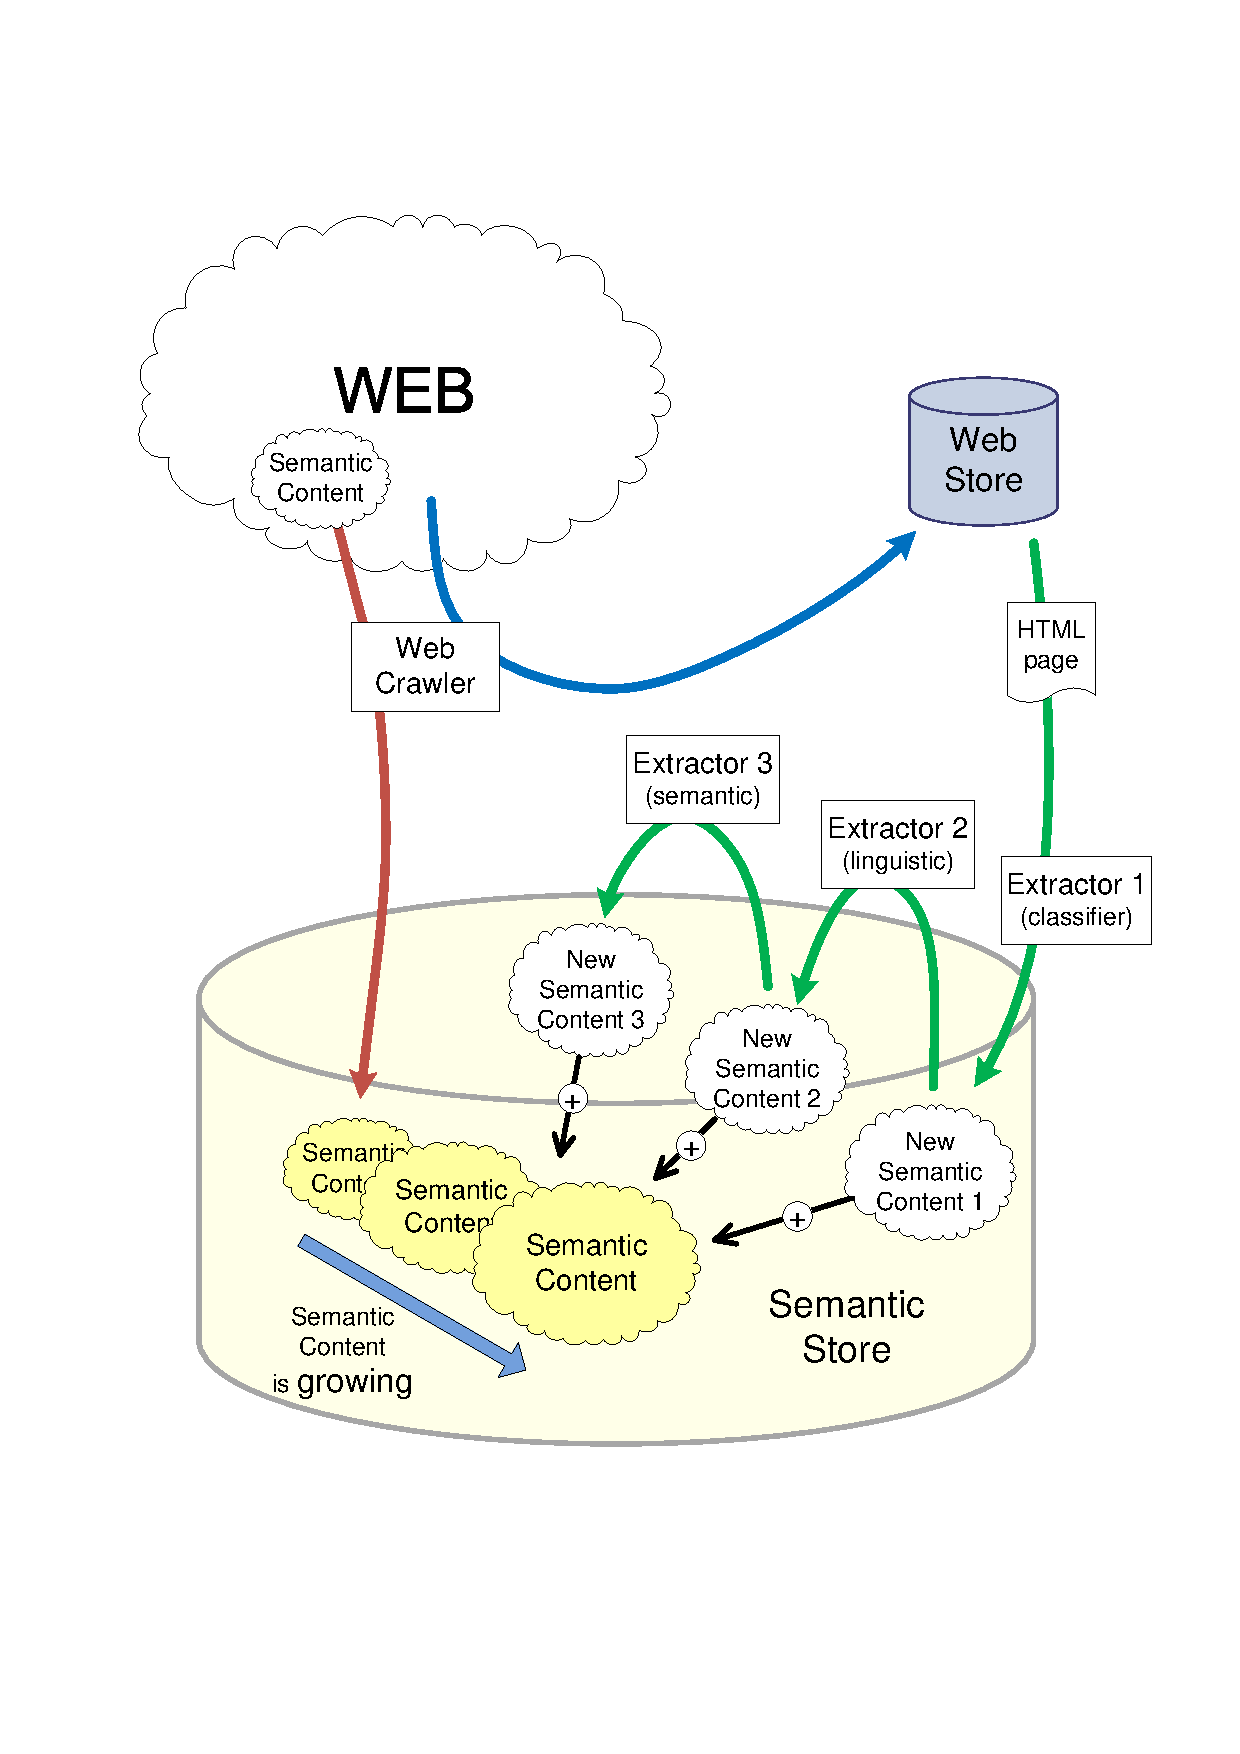
\includegraphics[height=0.5\vsize]{img/growing_semantization}
\end{columns}	
\end{frame}



%\begin{frame}{Available Resources and Allocated Capabilities}
%\begin{itemize}
	%\item Full time Ph.D. Student (4 years)
	%\begin{itemize}
		%\item In the beginning usually not yet skilled researcher in given topic
	%\end{itemize}	
	%\item Studying duties and activities
	%\begin{itemize}
		%\item There are so many interesting subjects not possible to attend because of lack of time 
	%\end{itemize}	
	%\item Teaching duties	
	%\begin{itemize}
		%\item Preparation of lecture materials
		%\item Student's homeworks, exams
	%\end{itemize}	
	%\item Writing papers 
	%\begin{itemize}
		%\item Not always completely relevant to the Ph.D. topic
	%\end{itemize}
	%\item Presentations, conferences
	%\begin{itemize}
		%\item Preparations
		%\item Traveling
	%\end{itemize}
	%\item Writing reviews 
	%\begin{itemize}
		%\item Student's thesis
		%\item Research papers
	%\end{itemize}
	%\item Internship?
	%\medskip
	%\item Active research
	%\begin{itemize}
		%\item Optimistic balance: remaining 30\% of available resources (not only time)
		%%\item Searching for existing approaches and studying them
		%%\item Working with new technologies
		%%\item Software development
	%\end{itemize}	
%\end{itemize}
%\end{frame}


\end{document}
